\documentclass[twoside]{book}

% Packages required by doxygen
\usepackage{fixltx2e}
\usepackage{calc}
\usepackage{doxygen}
\usepackage[export]{adjustbox} % also loads graphicx
\usepackage{graphicx}
\usepackage[utf8]{inputenc}
\usepackage{makeidx}
\usepackage{multicol}
\usepackage{multirow}
\PassOptionsToPackage{warn}{textcomp}
\usepackage{textcomp}
\usepackage[nointegrals]{wasysym}
\usepackage[table]{xcolor}

% NLS support packages
\usepackage[catalan]{babel}

% Font selection
\usepackage[T1]{fontenc}
\usepackage[scaled=.90]{helvet}
\usepackage{courier}
\usepackage{amssymb}
\usepackage{sectsty}
\renewcommand{\familydefault}{\sfdefault}
\allsectionsfont{%
  \fontseries{bc}\selectfont%
  \color{darkgray}%
}
\renewcommand{\DoxyLabelFont}{%
  \fontseries{bc}\selectfont%
  \color{darkgray}%
}
\newcommand{\+}{\discretionary{\mbox{\scriptsize$\hookleftarrow$}}{}{}}

% Page & text layout
\usepackage{geometry}
\geometry{%
  a4paper,%
  top=2.5cm,%
  bottom=2.5cm,%
  left=2.5cm,%
  right=2.5cm%
}
\tolerance=750
\hfuzz=15pt
\hbadness=750
\setlength{\emergencystretch}{15pt}
\setlength{\parindent}{0cm}
\setlength{\parskip}{3ex plus 2ex minus 2ex}
\makeatletter
\renewcommand{\paragraph}{%
  \@startsection{paragraph}{4}{0ex}{-1.0ex}{1.0ex}{%
    \normalfont\normalsize\bfseries\SS@parafont%
  }%
}
\renewcommand{\subparagraph}{%
  \@startsection{subparagraph}{5}{0ex}{-1.0ex}{1.0ex}{%
    \normalfont\normalsize\bfseries\SS@subparafont%
  }%
}
\makeatother

% Headers & footers
\usepackage{fancyhdr}
\pagestyle{fancyplain}
\fancyhead[LE]{\fancyplain{}{\bfseries\thepage}}
\fancyhead[CE]{\fancyplain{}{}}
\fancyhead[RE]{\fancyplain{}{\bfseries\leftmark}}
\fancyhead[LO]{\fancyplain{}{\bfseries\rightmark}}
\fancyhead[CO]{\fancyplain{}{}}
\fancyhead[RO]{\fancyplain{}{\bfseries\thepage}}
\fancyfoot[LE]{\fancyplain{}{}}
\fancyfoot[CE]{\fancyplain{}{}}
\fancyfoot[RE]{\fancyplain{}{\bfseries\scriptsize Generat per Doxygen }}
\fancyfoot[LO]{\fancyplain{}{\bfseries\scriptsize Generat per Doxygen }}
\fancyfoot[CO]{\fancyplain{}{}}
\fancyfoot[RO]{\fancyplain{}{}}
\renewcommand{\footrulewidth}{0.4pt}
\renewcommand{\chaptermark}[1]{%
  \markboth{#1}{}%
}
\renewcommand{\sectionmark}[1]{%
  \markright{\thesection\ #1}%
}

% Indices & bibliography
\usepackage{natbib}
\usepackage[titles]{tocloft}
\setcounter{tocdepth}{3}
\setcounter{secnumdepth}{5}
\makeindex

% Hyperlinks (required, but should be loaded last)
\usepackage{ifpdf}
\ifpdf
  \usepackage[pdftex,pagebackref=true]{hyperref}
\else
  \usepackage[ps2pdf,pagebackref=true]{hyperref}
\fi
\hypersetup{%
  colorlinks=true,%
  linkcolor=blue,%
  citecolor=blue,%
  unicode%
}

% Custom commands
\newcommand{\clearemptydoublepage}{%
  \newpage{\pagestyle{empty}\cleardoublepage}%
}

\usepackage{caption}
\captionsetup{labelsep=space,justification=centering,font={bf},singlelinecheck=off,skip=4pt,position=top}

%===== C O N T E N T S =====

\begin{document}

% Titlepage & ToC
\hypersetup{pageanchor=false,
             bookmarksnumbered=true,
             pdfencoding=unicode
            }
\pagenumbering{roman}
\begin{titlepage}
\vspace*{7cm}
\begin{center}%
{\Large Pràctica P\+R\+O2. Aplicació per a un laboratori de biologia. \\[1ex]\large 16-\/12-\/2017 }\\
\vspace*{1cm}
{\large Generat per Doxygen 1.8.11}\\
\end{center}
\end{titlepage}
\clearemptydoublepage
\tableofcontents
\clearemptydoublepage
\pagenumbering{arabic}
\hypersetup{pageanchor=true}

%--- Begin generated contents ---
\chapter{Pàgina principal}
\label{index}\hypertarget{index}{}En el mòdul \hyperlink{program_8cc}{program.\+cc} es troba el programa principal. Per l\textquotesingle{}aplicació per a un laboratori de biologia, necesitarem un mòdul per representa l\textquotesingle{}\hyperlink{class_individu}{Individu}, un altre pel posible \hyperlink{class_tret}{Tret}, a més de dos mòduls per a cada conjunt d\textquotesingle{}aquests, \hyperlink{class_cjt__individus}{Cjt\+\_\+individus} i \hyperlink{class_cjt__trets}{Cjt\+\_\+trets}, i finalment un mòdul \hyperlink{class_cromosomes}{Cromosomes}. 
\chapter{Índex de Classes}
\section{Llista de Classes}
Aquestes són les classes, estructures, unions i interfícies acompanyades amb breus descripcions\+:\begin{DoxyCompactList}
\item\contentsline{section}{\hyperlink{class_bin_tree}{Bin\+Tree$<$ T $>$} }{\pageref{class_bin_tree}}{}
\item\contentsline{section}{\hyperlink{class_cjt__individus}{Cjt\+\_\+individus} \\*Representa el conjunt d\textquotesingle{}individus d\textquotesingle{}un experiment }{\pageref{class_cjt__individus}}{}
\item\contentsline{section}{\hyperlink{class_cjt__trets}{Cjt\+\_\+trets} \\*Representa el conjunt de trets d\textquotesingle{}un experiment }{\pageref{class_cjt__trets}}{}
\item\contentsline{section}{\hyperlink{class_cromosomes}{Cromosomes} \\*Representa el parell de cromosomes }{\pageref{class_cromosomes}}{}
\item\contentsline{section}{\hyperlink{class_individu}{Individu} \\*Representa les característiques d\textquotesingle{}un individu }{\pageref{class_individu}}{}
\item\contentsline{section}{\hyperlink{struct_bin_tree_1_1_node}{Bin\+Tree$<$ T $>$\+::\+Node} }{\pageref{struct_bin_tree_1_1_node}}{}
\item\contentsline{section}{\hyperlink{class_tret}{Tret} \\*Representa l\textquotesingle{}informació i les operacions associades a un tret }{\pageref{class_tret}}{}
\end{DoxyCompactList}

\chapter{Índex de Fitxers}
\section{Llista dels Fitxers}
Aquesta és la llista de tots els fitxers acompanyats amb breus descripcions\+:\begin{DoxyCompactList}
\item\contentsline{section}{\hyperlink{_bin_tree_8hh}{Bin\+Tree.\+hh} }{\pageref{_bin_tree_8hh}}{}
\item\contentsline{section}{\hyperlink{_cjt__individus_8cc}{Cjt\+\_\+individus.\+cc} \\*Codi de la classe \hyperlink{class_cjt__individus}{Cjt\+\_\+individus} }{\pageref{_cjt__individus_8cc}}{}
\item\contentsline{section}{\hyperlink{_cjt__individus_8hh}{Cjt\+\_\+individus.\+hh} \\*Especificació de la classe \hyperlink{class_cjt__individus}{Cjt\+\_\+individus} }{\pageref{_cjt__individus_8hh}}{}
\item\contentsline{section}{\hyperlink{_cjt__trets_8cc}{Cjt\+\_\+trets.\+cc} \\*Codi de la classe \hyperlink{class_cjt__trets}{Cjt\+\_\+trets} }{\pageref{_cjt__trets_8cc}}{}
\item\contentsline{section}{\hyperlink{_cjt__trets_8hh}{Cjt\+\_\+trets.\+hh} \\*Especificació de la classe \hyperlink{class_cjt__trets}{Cjt\+\_\+trets} }{\pageref{_cjt__trets_8hh}}{}
\item\contentsline{section}{\hyperlink{_cromosomes_8cc}{Cromosomes.\+cc} \\*Codi de la classe \hyperlink{class_cromosomes}{Cromosomes} }{\pageref{_cromosomes_8cc}}{}
\item\contentsline{section}{\hyperlink{_cromosomes_8hh}{Cromosomes.\+hh} \\*Especificació de la classe \hyperlink{class_cromosomes}{Cromosomes} }{\pageref{_cromosomes_8hh}}{}
\item\contentsline{section}{\hyperlink{_individu_8cc}{Individu.\+cc} \\*Codi de la classe \hyperlink{class_individu}{Individu} }{\pageref{_individu_8cc}}{}
\item\contentsline{section}{\hyperlink{_individu_8hh}{Individu.\+hh} \\*Especificació de la classe \hyperlink{class_individu}{Individu} }{\pageref{_individu_8hh}}{}
\item\contentsline{section}{\hyperlink{program_8cc}{program.\+cc} \\*Programa principal {\itshape Aplicació per a un laboratori de biologia} }{\pageref{program_8cc}}{}
\item\contentsline{section}{\hyperlink{_tret_8cc}{Tret.\+cc} \\*Codi de la classe \hyperlink{class_tret}{Tret} }{\pageref{_tret_8cc}}{}
\item\contentsline{section}{\hyperlink{_tret_8hh}{Tret.\+hh} \\*Especificació de la classe \hyperlink{class_tret}{Tret} }{\pageref{_tret_8hh}}{}
\end{DoxyCompactList}

\chapter{Documentació de les Classes}
\hypertarget{class_bin_tree}{}\section{Referència de la Classe Template Bin\+Tree$<$ T $>$}
\label{class_bin_tree}\index{Bin\+Tree$<$ T $>$@{Bin\+Tree$<$ T $>$}}
\subsection*{Classes}
\begin{DoxyCompactItemize}
\item 
struct \hyperlink{struct_bin_tree_1_1_node}{Node}
\end{DoxyCompactItemize}
\subsection*{Mètodes públics}
\begin{DoxyCompactItemize}
\item 
\hyperlink{class_bin_tree_a47eef22d29cd023449d97c073c08e5b6}{Bin\+Tree} ()
\item 
\hyperlink{class_bin_tree_a1ab686e0bcf990093ff91fe71744c1a4}{Bin\+Tree} (const T \&x)
\item 
\hyperlink{class_bin_tree_adb7eeff76d08130c943b36af215eb521}{Bin\+Tree} (const T \&x, const \hyperlink{class_bin_tree}{Bin\+Tree} \&\hyperlink{class_bin_tree_a781025fb1c3693e91e851d55b181bedd}{left}, const \hyperlink{class_bin_tree}{Bin\+Tree} \&\hyperlink{class_bin_tree_a009c4bb95a25a1b639da637de32101ce}{right})
\item 
bool \hyperlink{class_bin_tree_a9ca8d7ae95b9bed51eb43f30c8d2bd58}{empty} () const 
\item 
\hyperlink{class_bin_tree}{Bin\+Tree} \hyperlink{class_bin_tree_a781025fb1c3693e91e851d55b181bedd}{left} () const 
\item 
\hyperlink{class_bin_tree}{Bin\+Tree} \hyperlink{class_bin_tree_a009c4bb95a25a1b639da637de32101ce}{right} () const 
\item 
const T \& \hyperlink{class_bin_tree_af545517333e94fdbfccfbc7df7d961fe}{value} () const 
\end{DoxyCompactItemize}
\subsection*{Mètodes Privats}
\begin{DoxyCompactItemize}
\item 
\hyperlink{class_bin_tree_a1408d37d1afda12d99747d09543c15f4}{Bin\+Tree} (shared\+\_\+ptr$<$ \hyperlink{struct_bin_tree_1_1_node}{Node} $>$ \hyperlink{class_bin_tree_afe3647af1dda90f6ddf1deee6560fcf1}{p})
\end{DoxyCompactItemize}
\subsection*{Atributs Privats}
\begin{DoxyCompactItemize}
\item 
shared\+\_\+ptr$<$ \hyperlink{struct_bin_tree_1_1_node}{Node} $>$ \hyperlink{class_bin_tree_afe3647af1dda90f6ddf1deee6560fcf1}{p}
\end{DoxyCompactItemize}


\subsection{Descripció Detallada}
\subsubsection*{template$<$typename T$>$\\*
class Bin\+Tree$<$ T $>$}



Definició a la línia 15 del fitxer Bin\+Tree.\+hh.



\subsection{Documentació del Constructor i el Destructor}
\index{Bin\+Tree@{Bin\+Tree}!Bin\+Tree@{Bin\+Tree}}
\index{Bin\+Tree@{Bin\+Tree}!Bin\+Tree@{Bin\+Tree}}
\subsubsection[{\texorpdfstring{Bin\+Tree(shared\+\_\+ptr$<$ Node $>$ p)}{BinTree(shared_ptr< Node > p)}}]{\setlength{\rightskip}{0pt plus 5cm}template$<$typename T$>$ {\bf Bin\+Tree}$<$ T $>$\+::{\bf Bin\+Tree} (
\begin{DoxyParamCaption}
\item[{shared\+\_\+ptr$<$ {\bf Node} $>$}]{p}
\end{DoxyParamCaption}
)\hspace{0.3cm}{\ttfamily [private]}}\hypertarget{class_bin_tree_a1408d37d1afda12d99747d09543c15f4}{}\label{class_bin_tree_a1408d37d1afda12d99747d09543c15f4}


Definició a la línia 32 del fitxer Bin\+Tree.\+hh.


\begin{DoxyCode}
33     :   \hyperlink{class_bin_tree_afe3647af1dda90f6ddf1deee6560fcf1}{p}(\hyperlink{class_bin_tree_afe3647af1dda90f6ddf1deee6560fcf1}{p})
34     \{   \}
\end{DoxyCode}
\index{Bin\+Tree@{Bin\+Tree}!Bin\+Tree@{Bin\+Tree}}
\index{Bin\+Tree@{Bin\+Tree}!Bin\+Tree@{Bin\+Tree}}
\subsubsection[{\texorpdfstring{Bin\+Tree()}{BinTree()}}]{\setlength{\rightskip}{0pt plus 5cm}template$<$typename T$>$ {\bf Bin\+Tree}$<$ T $>$\+::{\bf Bin\+Tree} (
\begin{DoxyParamCaption}
{}
\end{DoxyParamCaption}
)}\hypertarget{class_bin_tree_a47eef22d29cd023449d97c073c08e5b6}{}\label{class_bin_tree_a47eef22d29cd023449d97c073c08e5b6}


Definició a la línia 44 del fitxer Bin\+Tree.\+hh.


\begin{DoxyCode}
45     :   \hyperlink{class_bin_tree_afe3647af1dda90f6ddf1deee6560fcf1}{p}(\textcolor{keyword}{nullptr})
46     \{   \}
\end{DoxyCode}
\index{Bin\+Tree@{Bin\+Tree}!Bin\+Tree@{Bin\+Tree}}
\index{Bin\+Tree@{Bin\+Tree}!Bin\+Tree@{Bin\+Tree}}
\subsubsection[{\texorpdfstring{Bin\+Tree(const T \&x)}{BinTree(const T &x)}}]{\setlength{\rightskip}{0pt plus 5cm}template$<$typename T$>$ {\bf Bin\+Tree}$<$ T $>$\+::{\bf Bin\+Tree} (
\begin{DoxyParamCaption}
\item[{const T \&}]{x}
\end{DoxyParamCaption}
)}\hypertarget{class_bin_tree_a1ab686e0bcf990093ff91fe71744c1a4}{}\label{class_bin_tree_a1ab686e0bcf990093ff91fe71744c1a4}


Definició a la línia 49 del fitxer Bin\+Tree.\+hh.


\begin{DoxyCode}
49                          \{
50         \hyperlink{class_bin_tree_afe3647af1dda90f6ddf1deee6560fcf1}{p} = make\_shared<Node>(x, \textcolor{keyword}{nullptr}, \textcolor{keyword}{nullptr});
51     \}
\end{DoxyCode}
\index{Bin\+Tree@{Bin\+Tree}!Bin\+Tree@{Bin\+Tree}}
\index{Bin\+Tree@{Bin\+Tree}!Bin\+Tree@{Bin\+Tree}}
\subsubsection[{\texorpdfstring{Bin\+Tree(const T \&x, const Bin\+Tree \&left, const Bin\+Tree \&right)}{BinTree(const T &x, const BinTree &left, const BinTree &right)}}]{\setlength{\rightskip}{0pt plus 5cm}template$<$typename T$>$ {\bf Bin\+Tree}$<$ T $>$\+::{\bf Bin\+Tree} (
\begin{DoxyParamCaption}
\item[{const T \&}]{x, }
\item[{const {\bf Bin\+Tree}$<$ T $>$ \&}]{left, }
\item[{const {\bf Bin\+Tree}$<$ T $>$ \&}]{right}
\end{DoxyParamCaption}
)}\hypertarget{class_bin_tree_adb7eeff76d08130c943b36af215eb521}{}\label{class_bin_tree_adb7eeff76d08130c943b36af215eb521}


Definició a la línia 54 del fitxer Bin\+Tree.\+hh.


\begin{DoxyCode}
54                                                                     \{
55         \hyperlink{class_bin_tree_afe3647af1dda90f6ddf1deee6560fcf1}{p} = make\_shared<Node>(x, left.\hyperlink{class_bin_tree_afe3647af1dda90f6ddf1deee6560fcf1}{p}, right.\hyperlink{class_bin_tree_afe3647af1dda90f6ddf1deee6560fcf1}{p});
56     \}
\end{DoxyCode}


\subsection{Documentació de les Funcions Membre}
\index{Bin\+Tree@{Bin\+Tree}!empty@{empty}}
\index{empty@{empty}!Bin\+Tree@{Bin\+Tree}}
\subsubsection[{\texorpdfstring{empty() const }{empty() const }}]{\setlength{\rightskip}{0pt plus 5cm}template$<$typename T$>$ bool {\bf Bin\+Tree}$<$ T $>$\+::empty (
\begin{DoxyParamCaption}
{}
\end{DoxyParamCaption}
) const}\hypertarget{class_bin_tree_a9ca8d7ae95b9bed51eb43f30c8d2bd58}{}\label{class_bin_tree_a9ca8d7ae95b9bed51eb43f30c8d2bd58}


Definició a la línia 59 del fitxer Bin\+Tree.\+hh.


\begin{DoxyCode}
59                         \{
60         \textcolor{keywordflow}{return} not \hyperlink{class_bin_tree_afe3647af1dda90f6ddf1deee6560fcf1}{p};
61     \}
\end{DoxyCode}
\index{Bin\+Tree@{Bin\+Tree}!left@{left}}
\index{left@{left}!Bin\+Tree@{Bin\+Tree}}
\subsubsection[{\texorpdfstring{left() const }{left() const }}]{\setlength{\rightskip}{0pt plus 5cm}template$<$typename T$>$ {\bf Bin\+Tree} {\bf Bin\+Tree}$<$ T $>$\+::left (
\begin{DoxyParamCaption}
{}
\end{DoxyParamCaption}
) const}\hypertarget{class_bin_tree_a781025fb1c3693e91e851d55b181bedd}{}\label{class_bin_tree_a781025fb1c3693e91e851d55b181bedd}


Definició a la línia 64 del fitxer Bin\+Tree.\+hh.


\begin{DoxyCode}
64                           \{
65         assert(not \hyperlink{class_bin_tree_a9ca8d7ae95b9bed51eb43f30c8d2bd58}{empty}());
66         \textcolor{keywordflow}{return} \hyperlink{class_bin_tree_a47eef22d29cd023449d97c073c08e5b6}{BinTree}(\hyperlink{class_bin_tree_afe3647af1dda90f6ddf1deee6560fcf1}{p}->left);
67     \}
\end{DoxyCode}
\index{Bin\+Tree@{Bin\+Tree}!right@{right}}
\index{right@{right}!Bin\+Tree@{Bin\+Tree}}
\subsubsection[{\texorpdfstring{right() const }{right() const }}]{\setlength{\rightskip}{0pt plus 5cm}template$<$typename T$>$ {\bf Bin\+Tree} {\bf Bin\+Tree}$<$ T $>$\+::right (
\begin{DoxyParamCaption}
{}
\end{DoxyParamCaption}
) const}\hypertarget{class_bin_tree_a009c4bb95a25a1b639da637de32101ce}{}\label{class_bin_tree_a009c4bb95a25a1b639da637de32101ce}


Definició a la línia 70 del fitxer Bin\+Tree.\+hh.


\begin{DoxyCode}
70                            \{
71         assert(not \hyperlink{class_bin_tree_a9ca8d7ae95b9bed51eb43f30c8d2bd58}{empty}());
72         \textcolor{keywordflow}{return} \hyperlink{class_bin_tree_a47eef22d29cd023449d97c073c08e5b6}{BinTree}(\hyperlink{class_bin_tree_afe3647af1dda90f6ddf1deee6560fcf1}{p}->right);
73     \}
\end{DoxyCode}
\index{Bin\+Tree@{Bin\+Tree}!value@{value}}
\index{value@{value}!Bin\+Tree@{Bin\+Tree}}
\subsubsection[{\texorpdfstring{value() const }{value() const }}]{\setlength{\rightskip}{0pt plus 5cm}template$<$typename T$>$ const T\& {\bf Bin\+Tree}$<$ T $>$\+::value (
\begin{DoxyParamCaption}
{}
\end{DoxyParamCaption}
) const}\hypertarget{class_bin_tree_af545517333e94fdbfccfbc7df7d961fe}{}\label{class_bin_tree_af545517333e94fdbfccfbc7df7d961fe}


Definició a la línia 76 del fitxer Bin\+Tree.\+hh.


\begin{DoxyCode}
76                             \{
77         assert(not \hyperlink{class_bin_tree_a9ca8d7ae95b9bed51eb43f30c8d2bd58}{empty}());
78         \textcolor{keywordflow}{return} \hyperlink{class_bin_tree_afe3647af1dda90f6ddf1deee6560fcf1}{p}->x;
79     \}
\end{DoxyCode}


\subsection{Documentació de les Dades Membre}
\index{Bin\+Tree@{Bin\+Tree}!p@{p}}
\index{p@{p}!Bin\+Tree@{Bin\+Tree}}
\subsubsection[{\texorpdfstring{p}{p}}]{\setlength{\rightskip}{0pt plus 5cm}template$<$typename T$>$ shared\+\_\+ptr$<${\bf Node}$>$ {\bf Bin\+Tree}$<$ T $>$\+::p\hspace{0.3cm}{\ttfamily [private]}}\hypertarget{class_bin_tree_afe3647af1dda90f6ddf1deee6560fcf1}{}\label{class_bin_tree_afe3647af1dda90f6ddf1deee6560fcf1}


Definició a la línia 29 del fitxer Bin\+Tree.\+hh.



La documentació d\textquotesingle{}aquesta classe es va generar a partir del següent fitxer\+:\begin{DoxyCompactItemize}
\item 
\hyperlink{_bin_tree_8hh}{Bin\+Tree.\+hh}\end{DoxyCompactItemize}

\hypertarget{class_cjt__individus}{}\section{Referència de la Classe Cjt\+\_\+individus}
\label{class_cjt__individus}\index{Cjt\+\_\+individus@{Cjt\+\_\+individus}}


Representa el conjunt d\textquotesingle{}individus d\textquotesingle{}un experiment.  


\subsection*{Mètodes públics}
\begin{DoxyCompactItemize}
\item 
\hyperlink{class_cjt__individus_ace12a900a02d3b12c8067c7867618c50}{Cjt\+\_\+individus} ()
\begin{DoxyCompactList}\small\item\em Creadora per defecte. \end{DoxyCompactList}\item 
void \hyperlink{class_cjt__individus_a66d3e1b39b40532a2e2cff60fbf0b72a}{afegir\+\_\+tret} (int id, string tret)
\begin{DoxyCompactList}\small\item\em Modificadora dels individus que presenten el tret. \end{DoxyCompactList}\item 
void \hyperlink{class_cjt__individus_ab2f75f67eeaa424ffe8773e47d3223e8}{treure\+\_\+tret} (int id, string tret)
\begin{DoxyCompactList}\small\item\em Modificadora dels individus que presenten el tret. \end{DoxyCompactList}\item 
\hyperlink{class_cromosomes}{Cromosomes} \hyperlink{class_cjt__individus_a5c98261f78513b1b008cead471d8afa5}{consultar\+\_\+crom\+\_\+individu} (int id) const 
\begin{DoxyCompactList}\small\item\em Consulta els cromosomes d\textquotesingle{}un individu. \end{DoxyCompactList}\item 
bool \hyperlink{class_cjt__individus_ab7ef8ea63550958f2025a684dc804308}{individu\+\_\+te\+\_\+tret} (int id, string tret)
\begin{DoxyCompactList}\small\item\em Consulta si l\textquotesingle{}individu té el tret. \end{DoxyCompactList}\item 
void \hyperlink{class_cjt__individus_a478b829d6a11c5259a36a8bd53662e7d}{llegir} (int n, int m)
\begin{DoxyCompactList}\small\item\em Operació de lectura. \end{DoxyCompactList}\item 
void \hyperlink{class_cjt__individus_aafb2e0f4456390cbe83009aa542b0991}{escriure} (int id) const 
\begin{DoxyCompactList}\small\item\em Operació d\textquotesingle{}escriptura de l\textquotesingle{}individu. \end{DoxyCompactList}\item 
void \hyperlink{class_cjt__individus_afbd2a5f911caa9d9ca05470781c395a2}{escriure\+\_\+distribucio\+\_\+tret} (string tret)
\begin{DoxyCompactList}\small\item\em Operació d\textquotesingle{}escriptura de la distribució del tret. \end{DoxyCompactList}\end{DoxyCompactItemize}
\subsection*{Mètodes Privats}
\begin{DoxyCompactItemize}
\item 
void \hyperlink{class_cjt__individus_a569a1232f6660f888176cacd07df134a}{distribucio} (const \hyperlink{class_bin_tree}{Bin\+Tree}$<$ int $>$ \&a, \hyperlink{class_bin_tree}{Bin\+Tree}$<$ int $>$ \&dist, string tret)
\begin{DoxyCompactList}\small\item\em Operació que obté la distribució d\textquotesingle{}un tret. \end{DoxyCompactList}\end{DoxyCompactItemize}
\subsection*{Mètodes Privats Estàtics}
\begin{DoxyCompactItemize}
\item 
static void \hyperlink{class_cjt__individus_af4d73e9f298f7fab8411f2485a7c8fc5}{llegir\+\_\+arbre\+\_\+genealogic} (\hyperlink{class_bin_tree}{Bin\+Tree}$<$ int $>$ \&abregen)
\begin{DoxyCompactList}\small\item\em Operació de lectura de l\textquotesingle{}arbre genealògic. \end{DoxyCompactList}\item 
static void \hyperlink{class_cjt__individus_ac72868ef20cbed360206829ff580c38c}{escriure\+\_\+distribucio} (const \hyperlink{class_bin_tree}{Bin\+Tree}$<$ int $>$ \&dist)
\begin{DoxyCompactList}\small\item\em Operació d\textquotesingle{}escriptura de la distribució del tret. \end{DoxyCompactList}\end{DoxyCompactItemize}
\subsection*{Atributs Privats}
\begin{DoxyCompactItemize}
\item 
\hyperlink{class_bin_tree}{Bin\+Tree}$<$ int $>$ \hyperlink{class_cjt__individus_aa4786868783b8da4233a9b844ad376ce}{arbregen}
\begin{DoxyCompactList}\small\item\em Arbre genealogic, on cada node té l\textquotesingle{}identificador d\textquotesingle{}un individu. \end{DoxyCompactList}\item 
vector$<$ \hyperlink{class_individu}{Individu} $>$ \hyperlink{class_cjt__individus_aa28716121e4fbc5b6a90150748c9fc0b}{individus}
\begin{DoxyCompactList}\small\item\em Vector d\textquotesingle{}individus. \end{DoxyCompactList}\end{DoxyCompactItemize}


\subsection{Descripció Detallada}
Representa el conjunt d\textquotesingle{}individus d\textquotesingle{}un experiment. 

Ofereix operacions de lectura de l\textquotesingle{}experiment, escriptura i consultes d\textquotesingle{}un individu. 

Definició a la línia 24 del fitxer Cjt\+\_\+individus.\+hh.



\subsection{Documentació del Constructor i el Destructor}
\index{Cjt\+\_\+individus@{Cjt\+\_\+individus}!Cjt\+\_\+individus@{Cjt\+\_\+individus}}
\index{Cjt\+\_\+individus@{Cjt\+\_\+individus}!Cjt\+\_\+individus@{Cjt\+\_\+individus}}
\subsubsection[{\texorpdfstring{Cjt\+\_\+individus()}{Cjt_individus()}}]{\setlength{\rightskip}{0pt plus 5cm}Cjt\+\_\+individus\+::\+Cjt\+\_\+individus (
\begin{DoxyParamCaption}
{}
\end{DoxyParamCaption}
)}\hypertarget{class_cjt__individus_ace12a900a02d3b12c8067c7867618c50}{}\label{class_cjt__individus_ace12a900a02d3b12c8067c7867618c50}


Creadora per defecte. 

\begin{DoxyPrecond}{Precondició}
cert 
\end{DoxyPrecond}
\begin{DoxyPostcond}{Postcondició}
El resultat es un \hyperlink{class_cjt__individus}{Cjt\+\_\+individus} buit 
\end{DoxyPostcond}


Definició a la línia 7 del fitxer Cjt\+\_\+individus.\+cc.


\begin{DoxyCode}
7 \{\}
\end{DoxyCode}


\subsection{Documentació de les Funcions Membre}
\index{Cjt\+\_\+individus@{Cjt\+\_\+individus}!afegir\+\_\+tret@{afegir\+\_\+tret}}
\index{afegir\+\_\+tret@{afegir\+\_\+tret}!Cjt\+\_\+individus@{Cjt\+\_\+individus}}
\subsubsection[{\texorpdfstring{afegir\+\_\+tret(int id, string tret)}{afegir_tret(int id, string tret)}}]{\setlength{\rightskip}{0pt plus 5cm}void Cjt\+\_\+individus\+::afegir\+\_\+tret (
\begin{DoxyParamCaption}
\item[{int}]{id, }
\item[{string}]{tret}
\end{DoxyParamCaption}
)}\hypertarget{class_cjt__individus_a66d3e1b39b40532a2e2cff60fbf0b72a}{}\label{class_cjt__individus_a66d3e1b39b40532a2e2cff60fbf0b72a}


Modificadora dels individus que presenten el tret. 

\begin{DoxyPrecond}{Precondició}
cert 
\end{DoxyPrecond}
\begin{DoxyPostcond}{Postcondició}
S\textquotesingle{}afegeix el tret a l\textquotesingle{}individu 
\end{DoxyPostcond}


Definició a la línia 19 del fitxer Cjt\+\_\+individus.\+cc.


\begin{DoxyCode}
20 \{
21   \hyperlink{class_cjt__individus_aa28716121e4fbc5b6a90150748c9fc0b}{individus}[\textcolor{keywordtype}{id}-1].afegir(tret);
22 \}
\end{DoxyCode}
\index{Cjt\+\_\+individus@{Cjt\+\_\+individus}!treure\+\_\+tret@{treure\+\_\+tret}}
\index{treure\+\_\+tret@{treure\+\_\+tret}!Cjt\+\_\+individus@{Cjt\+\_\+individus}}
\subsubsection[{\texorpdfstring{treure\+\_\+tret(int id, string tret)}{treure_tret(int id, string tret)}}]{\setlength{\rightskip}{0pt plus 5cm}void Cjt\+\_\+individus\+::treure\+\_\+tret (
\begin{DoxyParamCaption}
\item[{int}]{id, }
\item[{string}]{tret}
\end{DoxyParamCaption}
)}\hypertarget{class_cjt__individus_ab2f75f67eeaa424ffe8773e47d3223e8}{}\label{class_cjt__individus_ab2f75f67eeaa424ffe8773e47d3223e8}


Modificadora dels individus que presenten el tret. 

\begin{DoxyPrecond}{Precondició}
cert 
\end{DoxyPrecond}
\begin{DoxyPostcond}{Postcondició}
Es treu el tret de l\textquotesingle{}individu 
\end{DoxyPostcond}


Definició a la línia 24 del fitxer Cjt\+\_\+individus.\+cc.


\begin{DoxyCode}
25 \{
26   \hyperlink{class_cjt__individus_aa28716121e4fbc5b6a90150748c9fc0b}{individus}[\textcolor{keywordtype}{id}-1].treure(tret);
27 \}
\end{DoxyCode}
\index{Cjt\+\_\+individus@{Cjt\+\_\+individus}!consultar\+\_\+crom\+\_\+individu@{consultar\+\_\+crom\+\_\+individu}}
\index{consultar\+\_\+crom\+\_\+individu@{consultar\+\_\+crom\+\_\+individu}!Cjt\+\_\+individus@{Cjt\+\_\+individus}}
\subsubsection[{\texorpdfstring{consultar\+\_\+crom\+\_\+individu(int id) const }{consultar_crom_individu(int id) const }}]{\setlength{\rightskip}{0pt plus 5cm}{\bf Cromosomes} Cjt\+\_\+individus\+::consultar\+\_\+crom\+\_\+individu (
\begin{DoxyParamCaption}
\item[{int}]{id}
\end{DoxyParamCaption}
) const}\hypertarget{class_cjt__individus_a5c98261f78513b1b008cead471d8afa5}{}\label{class_cjt__individus_a5c98261f78513b1b008cead471d8afa5}


Consulta els cromosomes d\textquotesingle{}un individu. 

\begin{DoxyPrecond}{Precondició}
cert 
\end{DoxyPrecond}
\begin{DoxyPostcond}{Postcondició}
Indica els cromosomes d\textquotesingle{}un individu 
\end{DoxyPostcond}


Definició a la línia 9 del fitxer Cjt\+\_\+individus.\+cc.


\begin{DoxyCode}
10 \{
11   \textcolor{keywordflow}{return} \hyperlink{class_cjt__individus_aa28716121e4fbc5b6a90150748c9fc0b}{individus}[\textcolor{keywordtype}{id}-1].consultar\_crom();
12 \}
\end{DoxyCode}
\index{Cjt\+\_\+individus@{Cjt\+\_\+individus}!individu\+\_\+te\+\_\+tret@{individu\+\_\+te\+\_\+tret}}
\index{individu\+\_\+te\+\_\+tret@{individu\+\_\+te\+\_\+tret}!Cjt\+\_\+individus@{Cjt\+\_\+individus}}
\subsubsection[{\texorpdfstring{individu\+\_\+te\+\_\+tret(int id, string tret)}{individu_te_tret(int id, string tret)}}]{\setlength{\rightskip}{0pt plus 5cm}bool Cjt\+\_\+individus\+::individu\+\_\+te\+\_\+tret (
\begin{DoxyParamCaption}
\item[{int}]{id, }
\item[{string}]{tret}
\end{DoxyParamCaption}
)}\hypertarget{class_cjt__individus_ab7ef8ea63550958f2025a684dc804308}{}\label{class_cjt__individus_ab7ef8ea63550958f2025a684dc804308}


Consulta si l\textquotesingle{}individu té el tret. 

\begin{DoxyPrecond}{Precondició}
cert 
\end{DoxyPrecond}
\begin{DoxyPostcond}{Postcondició}
Indica si presenta el tret 
\end{DoxyPostcond}


Definició a la línia 14 del fitxer Cjt\+\_\+individus.\+cc.


\begin{DoxyCode}
15 \{
16   \textcolor{keywordflow}{return} \hyperlink{class_cjt__individus_aa28716121e4fbc5b6a90150748c9fc0b}{individus}[\textcolor{keywordtype}{id}-1].te\_tret(tret);
17 \}
\end{DoxyCode}
\index{Cjt\+\_\+individus@{Cjt\+\_\+individus}!llegir@{llegir}}
\index{llegir@{llegir}!Cjt\+\_\+individus@{Cjt\+\_\+individus}}
\subsubsection[{\texorpdfstring{llegir(int n, int m)}{llegir(int n, int m)}}]{\setlength{\rightskip}{0pt plus 5cm}void Cjt\+\_\+individus\+::llegir (
\begin{DoxyParamCaption}
\item[{int}]{n, }
\item[{int}]{m}
\end{DoxyParamCaption}
)}\hypertarget{class_cjt__individus_a478b829d6a11c5259a36a8bd53662e7d}{}\label{class_cjt__individus_a478b829d6a11c5259a36a8bd53662e7d}


Operació de lectura. 

\begin{DoxyPrecond}{Precondició}
Estàn preparats al canal estàndard d\textquotesingle{}entrada un enter n $>$= 3, que representa el nombre d\textquotesingle{}individus, i el nombre de gens de cada cromosoma m $>$= 1 
\end{DoxyPrecond}
\begin{DoxyPostcond}{Postcondició}
El parametre implícit conté el conjunt d\textquotesingle{}individus llegit del canal estandard d\textquotesingle{}entrada 
\end{DoxyPostcond}


Definició a la línia 43 del fitxer Cjt\+\_\+individus.\+cc.


\begin{DoxyCode}
44 \{
45   \hyperlink{class_cjt__individus_aa28716121e4fbc5b6a90150748c9fc0b}{individus} = vector<Individu>(n);
46   \hyperlink{class_cjt__individus_af4d73e9f298f7fab8411f2485a7c8fc5}{llegir\_arbre\_genealogic}(\hyperlink{class_cjt__individus_aa4786868783b8da4233a9b844ad376ce}{arbregen});
47   \textcolor{keywordflow}{for}(\textcolor{keywordtype}{int} j = 0; j < n; ++j) \{
48     \hyperlink{class_individu}{Individu} x;
49     x.\hyperlink{class_individu_a03cd34a1eb0eaf4e0a1280ca8cc38a5f}{llegir\_individu}(m);
50     \hyperlink{class_cjt__individus_aa28716121e4fbc5b6a90150748c9fc0b}{individus}[j] = x;
51   \}
52 \}
\end{DoxyCode}
\index{Cjt\+\_\+individus@{Cjt\+\_\+individus}!escriure@{escriure}}
\index{escriure@{escriure}!Cjt\+\_\+individus@{Cjt\+\_\+individus}}
\subsubsection[{\texorpdfstring{escriure(int id) const }{escriure(int id) const }}]{\setlength{\rightskip}{0pt plus 5cm}void Cjt\+\_\+individus\+::escriure (
\begin{DoxyParamCaption}
\item[{int}]{id}
\end{DoxyParamCaption}
) const}\hypertarget{class_cjt__individus_aafb2e0f4456390cbe83009aa542b0991}{}\label{class_cjt__individus_aafb2e0f4456390cbe83009aa542b0991}


Operació d\textquotesingle{}escriptura de l\textquotesingle{}individu. 

\begin{DoxyPrecond}{Precondició}
cert 
\end{DoxyPrecond}
\begin{DoxyPostcond}{Postcondició}
S\textquotesingle{}escriu pel el canal de sortida estàndard l\textquotesingle{}individu 
\end{DoxyPostcond}


Definició a la línia 54 del fitxer Cjt\+\_\+individus.\+cc.


\begin{DoxyCode}
55 \{
56   \hyperlink{class_cjt__individus_aa28716121e4fbc5b6a90150748c9fc0b}{individus}[\textcolor{keywordtype}{id}-1].escriure\_individu();
57 \}
\end{DoxyCode}
\index{Cjt\+\_\+individus@{Cjt\+\_\+individus}!escriure\+\_\+distribucio\+\_\+tret@{escriure\+\_\+distribucio\+\_\+tret}}
\index{escriure\+\_\+distribucio\+\_\+tret@{escriure\+\_\+distribucio\+\_\+tret}!Cjt\+\_\+individus@{Cjt\+\_\+individus}}
\subsubsection[{\texorpdfstring{escriure\+\_\+distribucio\+\_\+tret(string tret)}{escriure_distribucio_tret(string tret)}}]{\setlength{\rightskip}{0pt plus 5cm}void Cjt\+\_\+individus\+::escriure\+\_\+distribucio\+\_\+tret (
\begin{DoxyParamCaption}
\item[{string}]{tret}
\end{DoxyParamCaption}
)}\hypertarget{class_cjt__individus_afbd2a5f911caa9d9ca05470781c395a2}{}\label{class_cjt__individus_afbd2a5f911caa9d9ca05470781c395a2}


Operació d\textquotesingle{}escriptura de la distribució del tret. 

\begin{DoxyPrecond}{Precondició}
cert 
\end{DoxyPrecond}
\begin{DoxyPostcond}{Postcondició}
S\textquotesingle{}escriu pel canal de sortida estàndard la distribució 
\end{DoxyPostcond}


Definició a la línia 92 del fitxer Cjt\+\_\+individus.\+cc.


\begin{DoxyCode}
93 \{
94   \hyperlink{class_bin_tree}{BinTree<int>} dist;
95   cout << \textcolor{stringliteral}{" "};
96   \hyperlink{class_cjt__individus_a569a1232f6660f888176cacd07df134a}{distribucio}(\hyperlink{class_cjt__individus_aa4786868783b8da4233a9b844ad376ce}{arbregen}, dist, tret);
97   \hyperlink{class_cjt__individus_ac72868ef20cbed360206829ff580c38c}{escriure\_distribucio}(dist);
98   cout << endl;
99 \}
\end{DoxyCode}
\index{Cjt\+\_\+individus@{Cjt\+\_\+individus}!llegir\+\_\+arbre\+\_\+genealogic@{llegir\+\_\+arbre\+\_\+genealogic}}
\index{llegir\+\_\+arbre\+\_\+genealogic@{llegir\+\_\+arbre\+\_\+genealogic}!Cjt\+\_\+individus@{Cjt\+\_\+individus}}
\subsubsection[{\texorpdfstring{llegir\+\_\+arbre\+\_\+genealogic(\+Bin\+Tree$<$ int $>$ \&abregen)}{llegir_arbre_genealogic(BinTree< int > &abregen)}}]{\setlength{\rightskip}{0pt plus 5cm}void Cjt\+\_\+individus\+::llegir\+\_\+arbre\+\_\+genealogic (
\begin{DoxyParamCaption}
\item[{{\bf Bin\+Tree}$<$ int $>$ \&}]{abregen}
\end{DoxyParamCaption}
)\hspace{0.3cm}{\ttfamily [static]}, {\ttfamily [private]}}\hypertarget{class_cjt__individus_af4d73e9f298f7fab8411f2485a7c8fc5}{}\label{class_cjt__individus_af4d73e9f298f7fab8411f2485a7c8fc5}


Operació de lectura de l\textquotesingle{}arbre genealògic. 

\begin{DoxyPrecond}{Precondició}
cert 
\end{DoxyPrecond}
\begin{DoxyPostcond}{Postcondició}
Es llegeix pel canal estàndard d\textquotesingle{}entrada la relació de parentiu i es forma l\textquotesingle{}arbre genealògic 
\end{DoxyPostcond}


Definició a la línia 29 del fitxer Cjt\+\_\+individus.\+cc.


\begin{DoxyCode}
30 \{
31 \textcolor{comment}{// Es llegeix l'abre en preordre}
32   \textcolor{keywordtype}{int} x;
33   cin >> x;
34   \textcolor{keywordflow}{if} (x!=0)\{
35     \hyperlink{class_bin_tree}{BinTree<int>} l;
36     \hyperlink{class_cjt__individus_af4d73e9f298f7fab8411f2485a7c8fc5}{llegir\_arbre\_genealogic}(l);
37     \hyperlink{class_bin_tree}{BinTree<int>} r;
38     \hyperlink{class_cjt__individus_af4d73e9f298f7fab8411f2485a7c8fc5}{llegir\_arbre\_genealogic}(r);
39     a=\hyperlink{class_bin_tree}{BinTree<int>}(x,l,r);
40   \}
41 \}
\end{DoxyCode}
\index{Cjt\+\_\+individus@{Cjt\+\_\+individus}!escriure\+\_\+distribucio@{escriure\+\_\+distribucio}}
\index{escriure\+\_\+distribucio@{escriure\+\_\+distribucio}!Cjt\+\_\+individus@{Cjt\+\_\+individus}}
\subsubsection[{\texorpdfstring{escriure\+\_\+distribucio(const Bin\+Tree$<$ int $>$ \&dist)}{escriure_distribucio(const BinTree< int > &dist)}}]{\setlength{\rightskip}{0pt plus 5cm}void Cjt\+\_\+individus\+::escriure\+\_\+distribucio (
\begin{DoxyParamCaption}
\item[{const {\bf Bin\+Tree}$<$ int $>$ \&}]{dist}
\end{DoxyParamCaption}
)\hspace{0.3cm}{\ttfamily [static]}, {\ttfamily [private]}}\hypertarget{class_cjt__individus_ac72868ef20cbed360206829ff580c38c}{}\label{class_cjt__individus_ac72868ef20cbed360206829ff580c38c}


Operació d\textquotesingle{}escriptura de la distribució del tret. 

\begin{DoxyPrecond}{Precondició}
cert 
\end{DoxyPrecond}
\begin{DoxyPostcond}{Postcondició}
S\textquotesingle{}escriu pel canal de sortida estàndard la distribució d\textquotesingle{}un tret en inordre 
\end{DoxyPostcond}


Definició a la línia 81 del fitxer Cjt\+\_\+individus.\+cc.


\begin{DoxyCode}
82 \{
83 \textcolor{comment}{// Escriu arbre en inordre}
84   \textcolor{keywordflow}{if} (not a.empty()) \{
85     \textcolor{keywordtype}{int} x = a.value();
86     \hyperlink{class_cjt__individus_ac72868ef20cbed360206829ff580c38c}{escriure\_distribucio}(a.left()); 
87     cout << \textcolor{stringliteral}{" "} << x;
88     \hyperlink{class_cjt__individus_ac72868ef20cbed360206829ff580c38c}{escriure\_distribucio}(a.right());
89   \}
90 \}
\end{DoxyCode}
\index{Cjt\+\_\+individus@{Cjt\+\_\+individus}!distribucio@{distribucio}}
\index{distribucio@{distribucio}!Cjt\+\_\+individus@{Cjt\+\_\+individus}}
\subsubsection[{\texorpdfstring{distribucio(const Bin\+Tree$<$ int $>$ \&a, Bin\+Tree$<$ int $>$ \&dist, string tret)}{distribucio(const BinTree< int > &a, BinTree< int > &dist, string tret)}}]{\setlength{\rightskip}{0pt plus 5cm}void Cjt\+\_\+individus\+::distribucio (
\begin{DoxyParamCaption}
\item[{const {\bf Bin\+Tree}$<$ int $>$ \&}]{a, }
\item[{{\bf Bin\+Tree}$<$ int $>$ \&}]{dist, }
\item[{string}]{tret}
\end{DoxyParamCaption}
)\hspace{0.3cm}{\ttfamily [private]}}\hypertarget{class_cjt__individus_a569a1232f6660f888176cacd07df134a}{}\label{class_cjt__individus_a569a1232f6660f888176cacd07df134a}


Operació que obté la distribució d\textquotesingle{}un tret. 

\begin{DoxyPrecond}{Precondició}
cert 
\end{DoxyPrecond}
\begin{DoxyPostcond}{Postcondició}
Es forma un nou subarbre de la distribució 
\end{DoxyPostcond}


Definició a la línia 59 del fitxer Cjt\+\_\+individus.\+cc.


\begin{DoxyCode}
60 \{
61   \textcolor{keywordflow}{if}(!a.\hyperlink{class_bin_tree_a9ca8d7ae95b9bed51eb43f30c8d2bd58}{empty}()) \{
62     \textcolor{keywordtype}{int} x = a.\hyperlink{class_bin_tree_af545517333e94fdbfccfbc7df7d961fe}{value}();
63     \textcolor{keywordflow}{if}(a.\hyperlink{class_bin_tree_a781025fb1c3693e91e851d55b181bedd}{left}().\hyperlink{class_bin_tree_a9ca8d7ae95b9bed51eb43f30c8d2bd58}{empty}()) \{\textcolor{comment}{// Fulla}
64       \textcolor{keywordflow}{if}(\hyperlink{class_cjt__individus_aa28716121e4fbc5b6a90150748c9fc0b}{individus}[x-1].te\_tret(tret)) dist = \hyperlink{class_bin_tree}{BinTree<int>}(x);
65       \textcolor{keywordflow}{else} dist = \hyperlink{class_bin_tree}{BinTree<int>}();
66     \}
67     \textcolor{keywordflow}{else} \{
68       \hyperlink{class_bin_tree}{BinTree<int>} l;
69       \hyperlink{class_bin_tree}{BinTree<int>} r;
70       \hyperlink{class_cjt__individus_a569a1232f6660f888176cacd07df134a}{distribucio}(a.\hyperlink{class_bin_tree_a781025fb1c3693e91e851d55b181bedd}{left}(),l,tret);
71       \hyperlink{class_cjt__individus_a569a1232f6660f888176cacd07df134a}{distribucio}(a.\hyperlink{class_bin_tree_a009c4bb95a25a1b639da637de32101ce}{right}(),r,tret);
72       \textcolor{keywordflow}{if}(\hyperlink{class_cjt__individus_aa28716121e4fbc5b6a90150748c9fc0b}{individus}[x-1].te\_tret(tret)) dist = \hyperlink{class_bin_tree}{BinTree<int>}(x, l, r);
73       \textcolor{keywordflow}{else} \{
74         \textcolor{keywordflow}{if}(l.\hyperlink{class_bin_tree_a9ca8d7ae95b9bed51eb43f30c8d2bd58}{empty}() and r.\hyperlink{class_bin_tree_a9ca8d7ae95b9bed51eb43f30c8d2bd58}{empty}()) dist=\hyperlink{class_bin_tree}{BinTree<int>}();\textcolor{comment}{// Si no té el tret i els
       progenitors tampoc llavors arbre buit}
75         \textcolor{keywordflow}{else} dist=\hyperlink{class_bin_tree}{BinTree<int>}(-x,l,r);\textcolor{comment}{// Si no té el tret pero si els progenitors llavors
       s'afegeix amb signe '-'}
76       \}
77     \}
78   \}
79 \}
\end{DoxyCode}


\subsection{Documentació de les Dades Membre}
\index{Cjt\+\_\+individus@{Cjt\+\_\+individus}!arbregen@{arbregen}}
\index{arbregen@{arbregen}!Cjt\+\_\+individus@{Cjt\+\_\+individus}}
\subsubsection[{\texorpdfstring{arbregen}{arbregen}}]{\setlength{\rightskip}{0pt plus 5cm}{\bf Bin\+Tree}$<$int$>$ Cjt\+\_\+individus\+::arbregen\hspace{0.3cm}{\ttfamily [private]}}\hypertarget{class_cjt__individus_aa4786868783b8da4233a9b844ad376ce}{}\label{class_cjt__individus_aa4786868783b8da4233a9b844ad376ce}


Arbre genealogic, on cada node té l\textquotesingle{}identificador d\textquotesingle{}un individu. 



Definició a la línia 29 del fitxer Cjt\+\_\+individus.\+hh.

\index{Cjt\+\_\+individus@{Cjt\+\_\+individus}!individus@{individus}}
\index{individus@{individus}!Cjt\+\_\+individus@{Cjt\+\_\+individus}}
\subsubsection[{\texorpdfstring{individus}{individus}}]{\setlength{\rightskip}{0pt plus 5cm}vector$<${\bf Individu}$>$ Cjt\+\_\+individus\+::individus\hspace{0.3cm}{\ttfamily [private]}}\hypertarget{class_cjt__individus_aa28716121e4fbc5b6a90150748c9fc0b}{}\label{class_cjt__individus_aa28716121e4fbc5b6a90150748c9fc0b}


Vector d\textquotesingle{}individus. 

Ordenat creixentment segons el seu identificador 

Definició a la línia 34 del fitxer Cjt\+\_\+individus.\+hh.



La documentació d\textquotesingle{}aquesta classe es va generar a partir dels següents fitxers\+:\begin{DoxyCompactItemize}
\item 
\hyperlink{_cjt__individus_8hh}{Cjt\+\_\+individus.\+hh}\item 
\hyperlink{_cjt__individus_8cc}{Cjt\+\_\+individus.\+cc}\end{DoxyCompactItemize}

\hypertarget{class_cjt__trets}{}\section{Referència de la Classe Cjt\+\_\+trets}
\label{class_cjt__trets}\index{Cjt\+\_\+trets@{Cjt\+\_\+trets}}


Representa el conjunt de trets d\textquotesingle{}un experiment.  


\subsection*{Mètodes públics}
\begin{DoxyCompactItemize}
\item 
\hyperlink{class_cjt__trets_a0f3d29b433ebfa6d9680e1ee0f39279b}{Cjt\+\_\+trets} ()
\begin{DoxyCompactList}\small\item\em Creadora per defecte. \end{DoxyCompactList}\item 
void \hyperlink{class_cjt__trets_ad315f780dfe22f6730ee9ce9aa2b25d7}{afegir} (string tret, int id, \hyperlink{class_cjt__individus}{Cjt\+\_\+individus} \&x)
\begin{DoxyCompactList}\small\item\em Modificadora del conjunt de trets. \end{DoxyCompactList}\item 
void \hyperlink{class_cjt__trets_ae4152db728b8c78d6e56856e0e88de33}{treure} (string tret, int id, \hyperlink{class_cjt__individus}{Cjt\+\_\+individus} \&x)
\begin{DoxyCompactList}\small\item\em Modificadora del conjunt de trets. \end{DoxyCompactList}\item 
bool \hyperlink{class_cjt__trets_a6da10e61a25071a25eca708f61a1e33d}{existeix\+\_\+tret} (string tret)
\begin{DoxyCompactList}\small\item\em Consulta si existeix el tret. \end{DoxyCompactList}\item 
void \hyperlink{class_cjt__trets_ad53ad0f5574d551fdbc8f665323a1db7}{escriure\+\_\+tret} (string tret)
\begin{DoxyCompactList}\small\item\em Operació d\textquotesingle{}escriptura del tret. \end{DoxyCompactList}\end{DoxyCompactItemize}
\subsection*{Atributs Privats}
\begin{DoxyCompactItemize}
\item 
map$<$ string, \hyperlink{class_tret}{Tret} $>$ \hyperlink{class_cjt__trets_ab13190e3207e0e51bd78cf16b8ed5360}{trets}
\begin{DoxyCompactList}\small\item\em Diccionari dels trets. \end{DoxyCompactList}\end{DoxyCompactItemize}


\subsection{Descripció Detallada}
Representa el conjunt de trets d\textquotesingle{}un experiment. 

Ofereix operacions per afegir, treure, consultar existencia i escriure trets. 

Definició a la línia 25 del fitxer Cjt\+\_\+trets.\+hh.



\subsection{Documentació del Constructor i el Destructor}
\index{Cjt\+\_\+trets@{Cjt\+\_\+trets}!Cjt\+\_\+trets@{Cjt\+\_\+trets}}
\index{Cjt\+\_\+trets@{Cjt\+\_\+trets}!Cjt\+\_\+trets@{Cjt\+\_\+trets}}
\subsubsection[{\texorpdfstring{Cjt\+\_\+trets()}{Cjt_trets()}}]{\setlength{\rightskip}{0pt plus 5cm}Cjt\+\_\+trets\+::\+Cjt\+\_\+trets (
\begin{DoxyParamCaption}
{}
\end{DoxyParamCaption}
)}\hypertarget{class_cjt__trets_a0f3d29b433ebfa6d9680e1ee0f39279b}{}\label{class_cjt__trets_a0f3d29b433ebfa6d9680e1ee0f39279b}


Creadora per defecte. 

\begin{DoxyPrecond}{Precondició}
cert 
\end{DoxyPrecond}
\begin{DoxyPostcond}{Postcondició}
El resultat es un \hyperlink{class_cjt__trets}{Cjt\+\_\+trets} buit 
\end{DoxyPostcond}


Definició a la línia 7 del fitxer Cjt\+\_\+trets.\+cc.


\begin{DoxyCode}
7 \{\}
\end{DoxyCode}


\subsection{Documentació de les Funcions Membre}
\index{Cjt\+\_\+trets@{Cjt\+\_\+trets}!afegir@{afegir}}
\index{afegir@{afegir}!Cjt\+\_\+trets@{Cjt\+\_\+trets}}
\subsubsection[{\texorpdfstring{afegir(string tret, int id, Cjt\+\_\+individus \&x)}{afegir(string tret, int id, Cjt_individus &x)}}]{\setlength{\rightskip}{0pt plus 5cm}void Cjt\+\_\+trets\+::afegir (
\begin{DoxyParamCaption}
\item[{string}]{tret, }
\item[{int}]{id, }
\item[{{\bf Cjt\+\_\+individus} \&}]{x}
\end{DoxyParamCaption}
)}\hypertarget{class_cjt__trets_ad315f780dfe22f6730ee9ce9aa2b25d7}{}\label{class_cjt__trets_ad315f780dfe22f6730ee9ce9aa2b25d7}


Modificadora del conjunt de trets. 

\begin{DoxyPrecond}{Precondició}
El tret no está present en el conjunt 
\end{DoxyPrecond}
\begin{DoxyPostcond}{Postcondició}
Si no hi era es crea, si hi era s\textquotesingle{}afegeix l\textquotesingle{}individu al tret 
\end{DoxyPostcond}


Definició a la línia 21 del fitxer Cjt\+\_\+trets.\+cc.


\begin{DoxyCode}
22 \{
23   x.\hyperlink{class_cjt__individus_a66d3e1b39b40532a2e2cff60fbf0b72a}{afegir\_tret}(\textcolor{keywordtype}{id}, tret);\textcolor{comment}{// S'afegeix el tret a l'individu}
24   \hyperlink{class_cjt__trets_ab13190e3207e0e51bd78cf16b8ed5360}{trets}[tret].afegir\_individu(\textcolor{keywordtype}{id}, x);\textcolor{comment}{// Si no existeix en el conjunt es crea}
25 \}
\end{DoxyCode}
\index{Cjt\+\_\+trets@{Cjt\+\_\+trets}!treure@{treure}}
\index{treure@{treure}!Cjt\+\_\+trets@{Cjt\+\_\+trets}}
\subsubsection[{\texorpdfstring{treure(string tret, int id, Cjt\+\_\+individus \&x)}{treure(string tret, int id, Cjt_individus &x)}}]{\setlength{\rightskip}{0pt plus 5cm}void Cjt\+\_\+trets\+::treure (
\begin{DoxyParamCaption}
\item[{string}]{tret, }
\item[{int}]{id, }
\item[{{\bf Cjt\+\_\+individus} \&}]{x}
\end{DoxyParamCaption}
)}\hypertarget{class_cjt__trets_ae4152db728b8c78d6e56856e0e88de33}{}\label{class_cjt__trets_ae4152db728b8c78d6e56856e0e88de33}


Modificadora del conjunt de trets. 

\begin{DoxyPrecond}{Precondició}
El tret está present en el conjunt 
\end{DoxyPrecond}
\begin{DoxyPostcond}{Postcondició}
Es treu l\textquotesingle{}individu del tret i si es qued buit s\textquotesingle{}elimina 
\end{DoxyPostcond}


Definició a la línia 27 del fitxer Cjt\+\_\+trets.\+cc.


\begin{DoxyCode}
28 \{
29   x.\hyperlink{class_cjt__individus_ab2f75f67eeaa424ffe8773e47d3223e8}{treure\_tret}(\textcolor{keywordtype}{id}, tret);\textcolor{comment}{// Es true el tret de l'individu}
30   \hyperlink{class_cjt__trets_ab13190e3207e0e51bd78cf16b8ed5360}{trets}[tret].treure\_individu(\textcolor{keywordtype}{id}, x);
31   \textcolor{keywordflow}{if}(\hyperlink{class_cjt__trets_ab13190e3207e0e51bd78cf16b8ed5360}{trets}[tret].buit()) \hyperlink{class_cjt__trets_ab13190e3207e0e51bd78cf16b8ed5360}{trets}.erase(tret);\textcolor{comment}{// Si el tret queda buit s'elimina}
32 \}
\end{DoxyCode}
\index{Cjt\+\_\+trets@{Cjt\+\_\+trets}!existeix\+\_\+tret@{existeix\+\_\+tret}}
\index{existeix\+\_\+tret@{existeix\+\_\+tret}!Cjt\+\_\+trets@{Cjt\+\_\+trets}}
\subsubsection[{\texorpdfstring{existeix\+\_\+tret(string tret)}{existeix_tret(string tret)}}]{\setlength{\rightskip}{0pt plus 5cm}bool Cjt\+\_\+trets\+::existeix\+\_\+tret (
\begin{DoxyParamCaption}
\item[{string}]{tret}
\end{DoxyParamCaption}
)}\hypertarget{class_cjt__trets_a6da10e61a25071a25eca708f61a1e33d}{}\label{class_cjt__trets_a6da10e61a25071a25eca708f61a1e33d}


Consulta si existeix el tret. 

\begin{DoxyPrecond}{Precondició}
cert 
\end{DoxyPrecond}
\begin{DoxyPostcond}{Postcondició}
Indica si existeix el tret 
\end{DoxyPostcond}


Definició a la línia 9 del fitxer Cjt\+\_\+trets.\+cc.


\begin{DoxyCode}
10 \{
11 \textcolor{comment}{// No es constant, ja que, al ser un diccionari si es consulta i no existeix es crea}
12   \textcolor{keywordtype}{bool} existeix = \textcolor{keyword}{true};
13   map<string, Tret>::const\_iterator it = \hyperlink{class_cjt__trets_ab13190e3207e0e51bd78cf16b8ed5360}{trets}.find(tret);
14   \textcolor{keywordflow}{if}(it == \hyperlink{class_cjt__trets_ab13190e3207e0e51bd78cf16b8ed5360}{trets}.end()) \{\textcolor{comment}{// Si no hi es s'elimina el tret creat al consultar}
15     existeix = \textcolor{keyword}{false};
16     \hyperlink{class_cjt__trets_ab13190e3207e0e51bd78cf16b8ed5360}{trets}.erase(tret);
17   \}
18   \textcolor{keywordflow}{return} existeix;
19 \}
\end{DoxyCode}
\index{Cjt\+\_\+trets@{Cjt\+\_\+trets}!escriure\+\_\+tret@{escriure\+\_\+tret}}
\index{escriure\+\_\+tret@{escriure\+\_\+tret}!Cjt\+\_\+trets@{Cjt\+\_\+trets}}
\subsubsection[{\texorpdfstring{escriure\+\_\+tret(string tret)}{escriure_tret(string tret)}}]{\setlength{\rightskip}{0pt plus 5cm}void Cjt\+\_\+trets\+::escriure\+\_\+tret (
\begin{DoxyParamCaption}
\item[{string}]{tret}
\end{DoxyParamCaption}
)}\hypertarget{class_cjt__trets_ad53ad0f5574d551fdbc8f665323a1db7}{}\label{class_cjt__trets_ad53ad0f5574d551fdbc8f665323a1db7}


Operació d\textquotesingle{}escriptura del tret. 

\begin{DoxyPrecond}{Precondició}
cert 
\end{DoxyPrecond}
\begin{DoxyPostcond}{Postcondició}
S\textquotesingle{}escriu pel el canal de sortida estàndard el tret 
\end{DoxyPostcond}


Definició a la línia 34 del fitxer Cjt\+\_\+trets.\+cc.


\begin{DoxyCode}
35 \{
36   cout << \textcolor{stringliteral}{"  "} << tret << endl;
37   \hyperlink{class_cjt__trets_ab13190e3207e0e51bd78cf16b8ed5360}{trets}[tret].escriure();
38 \}
\end{DoxyCode}


\subsection{Documentació de les Dades Membre}
\index{Cjt\+\_\+trets@{Cjt\+\_\+trets}!trets@{trets}}
\index{trets@{trets}!Cjt\+\_\+trets@{Cjt\+\_\+trets}}
\subsubsection[{\texorpdfstring{trets}{trets}}]{\setlength{\rightskip}{0pt plus 5cm}map$<$string, {\bf Tret}$>$ Cjt\+\_\+trets\+::trets\hspace{0.3cm}{\ttfamily [private]}}\hypertarget{class_cjt__trets_ab13190e3207e0e51bd78cf16b8ed5360}{}\label{class_cjt__trets_ab13190e3207e0e51bd78cf16b8ed5360}


Diccionari dels trets. 



Definició a la línia 31 del fitxer Cjt\+\_\+trets.\+hh.



La documentació d\textquotesingle{}aquesta classe es va generar a partir dels següents fitxers\+:\begin{DoxyCompactItemize}
\item 
\hyperlink{_cjt__trets_8hh}{Cjt\+\_\+trets.\+hh}\item 
\hyperlink{_cjt__trets_8cc}{Cjt\+\_\+trets.\+cc}\end{DoxyCompactItemize}

\hypertarget{class_cromosomes}{}\section{Referència de la Classe Cromosomes}
\label{class_cromosomes}\index{Cromosomes@{Cromosomes}}


Representa el parell de cromosomes.  


\subsection*{Mètodes públics}
\begin{DoxyCompactItemize}
\item 
\hyperlink{class_cromosomes_a117e49dbba6fef6e75d5ba774e1bd24a}{Cromosomes} ()
\begin{DoxyCompactList}\small\item\em Creador per defecte. \end{DoxyCompactList}\item 
void \hyperlink{class_cromosomes_a3453b58fad109a8317018f8349852d55}{combinacio\+\_\+crom} (const \hyperlink{class_cromosomes}{Cromosomes} \&x)
\begin{DoxyCompactList}\small\item\em Modificadora els cromosomes. \end{DoxyCompactList}\item 
void \hyperlink{class_cromosomes_ae475f91a7ebbe2b6253f2cf87e05d05c}{llegir\+\_\+cromosomes} (int m)
\begin{DoxyCompactList}\small\item\em Operació de lectura. \end{DoxyCompactList}\item 
void \hyperlink{class_cromosomes_a82634290c5bd73c827034902404c90cf}{escriure\+\_\+cromosomes} () const 
\begin{DoxyCompactList}\small\item\em Operació de escriptura. \end{DoxyCompactList}\end{DoxyCompactItemize}
\subsection*{Atributs Privats}
\begin{DoxyCompactItemize}
\item 
vector$<$ char $>$ \hyperlink{class_cromosomes_a663df9407657383482e40832eca6e91a}{crom}
\begin{DoxyCompactList}\small\item\em Vector del parell de cromosomes. \end{DoxyCompactList}\end{DoxyCompactItemize}


\subsection{Descripció Detallada}
Representa el parell de cromosomes. 

Conté els cromosomes i operacions per tratar-\/los. 

Definició a la línia 25 del fitxer Cromosomes.\+hh.



\subsection{Documentació del Constructor i el Destructor}
\index{Cromosomes@{Cromosomes}!Cromosomes@{Cromosomes}}
\index{Cromosomes@{Cromosomes}!Cromosomes@{Cromosomes}}
\subsubsection[{\texorpdfstring{Cromosomes()}{Cromosomes()}}]{\setlength{\rightskip}{0pt plus 5cm}Cromosomes\+::\+Cromosomes (
\begin{DoxyParamCaption}
{}
\end{DoxyParamCaption}
)}\hypertarget{class_cromosomes_a117e49dbba6fef6e75d5ba774e1bd24a}{}\label{class_cromosomes_a117e49dbba6fef6e75d5ba774e1bd24a}


Creador per defecte. 

\begin{DoxyPrecond}{Precondició}
cert 
\end{DoxyPrecond}
\begin{DoxyPostcond}{Postcondició}
El resultat es un vector de cromosomes buit 
\end{DoxyPostcond}


Definició a la línia 7 del fitxer Cromosomes.\+cc.


\begin{DoxyCode}
7 \{\}
\end{DoxyCode}


\subsection{Documentació de les Funcions Membre}
\index{Cromosomes@{Cromosomes}!combinacio\+\_\+crom@{combinacio\+\_\+crom}}
\index{combinacio\+\_\+crom@{combinacio\+\_\+crom}!Cromosomes@{Cromosomes}}
\subsubsection[{\texorpdfstring{combinacio\+\_\+crom(const Cromosomes \&x)}{combinacio_crom(const Cromosomes &x)}}]{\setlength{\rightskip}{0pt plus 5cm}void Cromosomes\+::combinacio\+\_\+crom (
\begin{DoxyParamCaption}
\item[{const {\bf Cromosomes} \&}]{x}
\end{DoxyParamCaption}
)}\hypertarget{class_cromosomes_a3453b58fad109a8317018f8349852d55}{}\label{class_cromosomes_a3453b58fad109a8317018f8349852d55}


Modificadora els cromosomes. 

\begin{DoxyPrecond}{Precondició}
cert 
\end{DoxyPrecond}
\begin{DoxyPostcond}{Postcondició}
El parametre implicit conté la intersecció del seu vector i el passar per paràmetre 
\end{DoxyPostcond}


Definició a la línia 9 del fitxer Cromosomes.\+cc.


\begin{DoxyCode}
10 \{
11   vector<char> comb;
12   comb = x.\hyperlink{class_cromosomes_a663df9407657383482e40832eca6e91a}{crom};
13   \textcolor{keywordtype}{int} tam = (\hyperlink{class_cromosomes_a663df9407657383482e40832eca6e91a}{crom}.size())/2;
14   \textcolor{keywordtype}{int} i = 0;
15   \textcolor{keywordflow}{while}(i<tam) \{
16     \textcolor{keywordflow}{if}((\hyperlink{class_cromosomes_a663df9407657383482e40832eca6e91a}{crom}[i] != comb[i]) or (\hyperlink{class_cromosomes_a663df9407657383482e40832eca6e91a}{crom}[tam+i] != comb[tam+i])) \{
17       \hyperlink{class_cromosomes_a663df9407657383482e40832eca6e91a}{crom}[i] = \textcolor{charliteral}{'-'};
18       \hyperlink{class_cromosomes_a663df9407657383482e40832eca6e91a}{crom}[tam+i] = \textcolor{charliteral}{'-'};  
19     \}
20     ++i;
21   \}
22 \}
\end{DoxyCode}
\index{Cromosomes@{Cromosomes}!llegir\+\_\+cromosomes@{llegir\+\_\+cromosomes}}
\index{llegir\+\_\+cromosomes@{llegir\+\_\+cromosomes}!Cromosomes@{Cromosomes}}
\subsubsection[{\texorpdfstring{llegir\+\_\+cromosomes(int m)}{llegir_cromosomes(int m)}}]{\setlength{\rightskip}{0pt plus 5cm}void Cromosomes\+::llegir\+\_\+cromosomes (
\begin{DoxyParamCaption}
\item[{int}]{m}
\end{DoxyParamCaption}
)}\hypertarget{class_cromosomes_ae475f91a7ebbe2b6253f2cf87e05d05c}{}\label{class_cromosomes_ae475f91a7ebbe2b6253f2cf87e05d05c}


Operació de lectura. 

\begin{DoxyPrecond}{Precondició}
cert 
\end{DoxyPrecond}
\begin{DoxyPostcond}{Postcondició}
El parametre implícit conté el vector de cromosomes llegit del canal estandard d\textquotesingle{}entrada 
\end{DoxyPostcond}


Definició a la línia 24 del fitxer Cromosomes.\+cc.


\begin{DoxyCode}
25 \{
26 \textcolor{comment}{// Esl parell de cromosomes es llegeix com a un únic vector, més fàcil de tractar,}
27 \textcolor{comment}{// i com es té un parell el tamany del vector sempre serà parell.}
28   \textcolor{keywordtype}{int} tam = 2*m;
29   \hyperlink{class_cromosomes_a663df9407657383482e40832eca6e91a}{crom} = vector<char>(tam);
30   \textcolor{keywordflow}{for} (\textcolor{keywordtype}{int} i = 0; i < tam; ++i) cin >> \hyperlink{class_cromosomes_a663df9407657383482e40832eca6e91a}{crom}[i];
31 \}
\end{DoxyCode}
\index{Cromosomes@{Cromosomes}!escriure\+\_\+cromosomes@{escriure\+\_\+cromosomes}}
\index{escriure\+\_\+cromosomes@{escriure\+\_\+cromosomes}!Cromosomes@{Cromosomes}}
\subsubsection[{\texorpdfstring{escriure\+\_\+cromosomes() const }{escriure_cromosomes() const }}]{\setlength{\rightskip}{0pt plus 5cm}void Cromosomes\+::escriure\+\_\+cromosomes (
\begin{DoxyParamCaption}
{}
\end{DoxyParamCaption}
) const}\hypertarget{class_cromosomes_a82634290c5bd73c827034902404c90cf}{}\label{class_cromosomes_a82634290c5bd73c827034902404c90cf}


Operació de escriptura. 

\begin{DoxyPrecond}{Precondició}
cert 
\end{DoxyPrecond}
\begin{DoxyPostcond}{Postcondició}
S\textquotesingle{}escriu pel el canal de sortida estàndard el vector de cromosomes 
\end{DoxyPostcond}


Definició a la línia 33 del fitxer Cromosomes.\+cc.


\begin{DoxyCode}
34 \{
35 \textcolor{comment}{// S'esecriu el vector en dos meitats, és a dir, el parell de cromosomes}
36   \textcolor{keywordtype}{int} tam = \hyperlink{class_cromosomes_a663df9407657383482e40832eca6e91a}{crom}.size();
37   \textcolor{keywordtype}{int} i = 0;
38   cout << \textcolor{stringliteral}{"  "};
39   \textcolor{keywordflow}{while} (i < tam/2) \{
40     cout << \hyperlink{class_cromosomes_a663df9407657383482e40832eca6e91a}{crom}[i];
41     ++i;
42   \}
43   cout << endl;
44   cout << \textcolor{stringliteral}{"  "};
45   \textcolor{keywordflow}{while}(i < tam) \{
46     cout << \hyperlink{class_cromosomes_a663df9407657383482e40832eca6e91a}{crom}[i];
47     ++i;  
48   \}
49   cout << endl;
50 \}
\end{DoxyCode}


\subsection{Documentació de les Dades Membre}
\index{Cromosomes@{Cromosomes}!crom@{crom}}
\index{crom@{crom}!Cromosomes@{Cromosomes}}
\subsubsection[{\texorpdfstring{crom}{crom}}]{\setlength{\rightskip}{0pt plus 5cm}vector$<$char$>$ Cromosomes\+::crom\hspace{0.3cm}{\ttfamily [private]}}\hypertarget{class_cromosomes_a663df9407657383482e40832eca6e91a}{}\label{class_cromosomes_a663df9407657383482e40832eca6e91a}


Vector del parell de cromosomes. 



Definició a la línia 30 del fitxer Cromosomes.\+hh.



La documentació d\textquotesingle{}aquesta classe es va generar a partir dels següents fitxers\+:\begin{DoxyCompactItemize}
\item 
\hyperlink{_cromosomes_8hh}{Cromosomes.\+hh}\item 
\hyperlink{_cromosomes_8cc}{Cromosomes.\+cc}\end{DoxyCompactItemize}

\hypertarget{class_individu}{}\section{Referència de la Classe Individu}
\label{class_individu}\index{Individu@{Individu}}


Representa les característiques d\textquotesingle{}un individu.  


\subsection*{Mètodes públics}
\begin{DoxyCompactItemize}
\item 
\hyperlink{class_individu_ac35091404cfbf11946694806aefa9e7e}{Individu} ()
\begin{DoxyCompactList}\small\item\em Creador per defecte. \end{DoxyCompactList}\item 
void \hyperlink{class_individu_a09f3188549ab207ae329ddf56ae6240f}{afegir} (string tret)
\begin{DoxyCompactList}\small\item\em Modificadora dels trets que presenta l\textquotesingle{}individu. \end{DoxyCompactList}\item 
void \hyperlink{class_individu_a8fbb728841cf4aefd304e10f4a6336a0}{treure} (string tret)
\begin{DoxyCompactList}\small\item\em Modificadora dels trets que presenta l\textquotesingle{}individu. \end{DoxyCompactList}\item 
\hyperlink{class_cromosomes}{Cromosomes} \hyperlink{class_individu_a39942c24ef726105afe2b193494985a0}{consultar\+\_\+crom} () const 
\begin{DoxyCompactList}\small\item\em Consulta els cromosomes de l\textquotesingle{}individu. \end{DoxyCompactList}\item 
bool \hyperlink{class_individu_a06cdcd2074fcf08fe55fe1e5014cd51b}{te\+\_\+tret} (string tret)
\begin{DoxyCompactList}\small\item\em Consulta si l\textquotesingle{}individu presenta el tret. \end{DoxyCompactList}\item 
void \hyperlink{class_individu_a03cd34a1eb0eaf4e0a1280ca8cc38a5f}{llegir\+\_\+individu} (int m)
\begin{DoxyCompactList}\small\item\em Operació de lectura. \end{DoxyCompactList}\item 
void \hyperlink{class_individu_af58b5637967c9ae9e27e62d5671d80a1}{escriure\+\_\+individu} () const 
\begin{DoxyCompactList}\small\item\em Operació de escriptura. \end{DoxyCompactList}\end{DoxyCompactItemize}
\subsection*{Atributs Privats}
\begin{DoxyCompactItemize}
\item 
\hyperlink{class_cromosomes}{Cromosomes} \hyperlink{class_individu_a84ba8716c5c488ea4be7b7218bde1b93}{crom}
\begin{DoxyCompactList}\small\item\em \hyperlink{class_cromosomes}{Cromosomes} de l\textquotesingle{}individu. \end{DoxyCompactList}\item 
set$<$ string $>$ \hyperlink{class_individu_a0ac8e4f21a7d491e6c8b90f267065bca}{trets}
\begin{DoxyCompactList}\small\item\em Conjunt dels trets que presenta. \end{DoxyCompactList}\end{DoxyCompactItemize}


\subsection{Descripció Detallada}
Representa les característiques d\textquotesingle{}un individu. 

Conté informació sobre l\textquotesingle{}individu, el parell de gens i els trets que presenta. 

Definició a la línia 24 del fitxer Individu.\+hh.



\subsection{Documentació del Constructor i el Destructor}
\index{Individu@{Individu}!Individu@{Individu}}
\index{Individu@{Individu}!Individu@{Individu}}
\subsubsection[{\texorpdfstring{Individu()}{Individu()}}]{\setlength{\rightskip}{0pt plus 5cm}Individu\+::\+Individu (
\begin{DoxyParamCaption}
{}
\end{DoxyParamCaption}
)}\hypertarget{class_individu_ac35091404cfbf11946694806aefa9e7e}{}\label{class_individu_ac35091404cfbf11946694806aefa9e7e}


Creador per defecte. 

\begin{DoxyPrecond}{Precondició}
cert 
\end{DoxyPrecond}
\begin{DoxyPostcond}{Postcondició}
El resultat es un individu buit 
\end{DoxyPostcond}


Definició a la línia 7 del fitxer Individu.\+cc.


\begin{DoxyCode}
7 \{\}
\end{DoxyCode}


\subsection{Documentació de les Funcions Membre}
\index{Individu@{Individu}!afegir@{afegir}}
\index{afegir@{afegir}!Individu@{Individu}}
\subsubsection[{\texorpdfstring{afegir(string tret)}{afegir(string tret)}}]{\setlength{\rightskip}{0pt plus 5cm}void Individu\+::afegir (
\begin{DoxyParamCaption}
\item[{string}]{tret}
\end{DoxyParamCaption}
)}\hypertarget{class_individu_a09f3188549ab207ae329ddf56ae6240f}{}\label{class_individu_a09f3188549ab207ae329ddf56ae6240f}


Modificadora dels trets que presenta l\textquotesingle{}individu. 

\begin{DoxyPrecond}{Precondició}
L\textquotesingle{}individu no presenta el tret 
\end{DoxyPrecond}
\begin{DoxyPostcond}{Postcondició}
S\textquotesingle{}afegeix el tret a l\textquotesingle{}individu 
\end{DoxyPostcond}


Definició a la línia 26 del fitxer Individu.\+cc.


\begin{DoxyCode}
27 \{
28   \hyperlink{class_individu_a0ac8e4f21a7d491e6c8b90f267065bca}{trets}.insert(tret);
29 \}
\end{DoxyCode}
\index{Individu@{Individu}!treure@{treure}}
\index{treure@{treure}!Individu@{Individu}}
\subsubsection[{\texorpdfstring{treure(string tret)}{treure(string tret)}}]{\setlength{\rightskip}{0pt plus 5cm}void Individu\+::treure (
\begin{DoxyParamCaption}
\item[{string}]{tret}
\end{DoxyParamCaption}
)}\hypertarget{class_individu_a8fbb728841cf4aefd304e10f4a6336a0}{}\label{class_individu_a8fbb728841cf4aefd304e10f4a6336a0}


Modificadora dels trets que presenta l\textquotesingle{}individu. 

\begin{DoxyPrecond}{Precondició}
L\textquotesingle{}individu presenta el tret 
\end{DoxyPrecond}
\begin{DoxyPostcond}{Postcondició}
Es treu el tret de l\textquotesingle{}individu 
\end{DoxyPostcond}


Definició a la línia 31 del fitxer Individu.\+cc.


\begin{DoxyCode}
32 \{
33   \hyperlink{class_individu_a0ac8e4f21a7d491e6c8b90f267065bca}{trets}.erase(tret);
34 \}
\end{DoxyCode}
\index{Individu@{Individu}!consultar\+\_\+crom@{consultar\+\_\+crom}}
\index{consultar\+\_\+crom@{consultar\+\_\+crom}!Individu@{Individu}}
\subsubsection[{\texorpdfstring{consultar\+\_\+crom() const }{consultar_crom() const }}]{\setlength{\rightskip}{0pt plus 5cm}{\bf Cromosomes} Individu\+::consultar\+\_\+crom (
\begin{DoxyParamCaption}
{}
\end{DoxyParamCaption}
) const}\hypertarget{class_individu_a39942c24ef726105afe2b193494985a0}{}\label{class_individu_a39942c24ef726105afe2b193494985a0}


Consulta els cromosomes de l\textquotesingle{}individu. 

\begin{DoxyPrecond}{Precondició}
cert 
\end{DoxyPrecond}
\begin{DoxyPostcond}{Postcondició}
Indica els cromosomes 
\end{DoxyPostcond}


Definició a la línia 9 del fitxer Individu.\+cc.


\begin{DoxyCode}
10 \{
11   \textcolor{keywordflow}{return} \hyperlink{class_individu_a84ba8716c5c488ea4be7b7218bde1b93}{crom};
12 \}
\end{DoxyCode}
\index{Individu@{Individu}!te\+\_\+tret@{te\+\_\+tret}}
\index{te\+\_\+tret@{te\+\_\+tret}!Individu@{Individu}}
\subsubsection[{\texorpdfstring{te\+\_\+tret(string tret)}{te_tret(string tret)}}]{\setlength{\rightskip}{0pt plus 5cm}bool Individu\+::te\+\_\+tret (
\begin{DoxyParamCaption}
\item[{string}]{tret}
\end{DoxyParamCaption}
)}\hypertarget{class_individu_a06cdcd2074fcf08fe55fe1e5014cd51b}{}\label{class_individu_a06cdcd2074fcf08fe55fe1e5014cd51b}


Consulta si l\textquotesingle{}individu presenta el tret. 

\begin{DoxyPrecond}{Precondició}
cert 
\end{DoxyPrecond}
\begin{DoxyPostcond}{Postcondició}
Indica si presenta el tret 
\end{DoxyPostcond}


Definició a la línia 14 del fitxer Individu.\+cc.


\begin{DoxyCode}
15 \{
16 \textcolor{comment}{// No es constant, ja que, al ser un conjunt si es consulta i no existeix es crea}
17   \textcolor{keywordtype}{bool} te = \textcolor{keyword}{true};
18   set<string>::const\_iterator it = \hyperlink{class_individu_a0ac8e4f21a7d491e6c8b90f267065bca}{trets}.find(tret);
19   \textcolor{keywordflow}{if}(it == \hyperlink{class_individu_a0ac8e4f21a7d491e6c8b90f267065bca}{trets}.end()) \{
20     te = \textcolor{keyword}{false};
21     \hyperlink{class_individu_a0ac8e4f21a7d491e6c8b90f267065bca}{trets}.erase(tret);
22   \}
23   \textcolor{keywordflow}{return} te;
24 \}
\end{DoxyCode}
\index{Individu@{Individu}!llegir\+\_\+individu@{llegir\+\_\+individu}}
\index{llegir\+\_\+individu@{llegir\+\_\+individu}!Individu@{Individu}}
\subsubsection[{\texorpdfstring{llegir\+\_\+individu(int m)}{llegir_individu(int m)}}]{\setlength{\rightskip}{0pt plus 5cm}void Individu\+::llegir\+\_\+individu (
\begin{DoxyParamCaption}
\item[{int}]{m}
\end{DoxyParamCaption}
)}\hypertarget{class_individu_a03cd34a1eb0eaf4e0a1280ca8cc38a5f}{}\label{class_individu_a03cd34a1eb0eaf4e0a1280ca8cc38a5f}


Operació de lectura. 

\begin{DoxyPrecond}{Precondició}
cert 
\end{DoxyPrecond}
\begin{DoxyPostcond}{Postcondició}
El parametre implicit conté els cromosomes d\textquotesingle{}aquest 
\end{DoxyPostcond}


Definició a la línia 36 del fitxer Individu.\+cc.


\begin{DoxyCode}
37 \{
38   \hyperlink{class_individu_a84ba8716c5c488ea4be7b7218bde1b93}{crom}.\hyperlink{class_cromosomes_ae475f91a7ebbe2b6253f2cf87e05d05c}{llegir\_cromosomes}(m);
39 \}
\end{DoxyCode}
\index{Individu@{Individu}!escriure\+\_\+individu@{escriure\+\_\+individu}}
\index{escriure\+\_\+individu@{escriure\+\_\+individu}!Individu@{Individu}}
\subsubsection[{\texorpdfstring{escriure\+\_\+individu() const }{escriure_individu() const }}]{\setlength{\rightskip}{0pt plus 5cm}void Individu\+::escriure\+\_\+individu (
\begin{DoxyParamCaption}
{}
\end{DoxyParamCaption}
) const}\hypertarget{class_individu_af58b5637967c9ae9e27e62d5671d80a1}{}\label{class_individu_af58b5637967c9ae9e27e62d5671d80a1}


Operació de escriptura. 

\begin{DoxyPrecond}{Precondició}
cert 
\end{DoxyPrecond}
\begin{DoxyPostcond}{Postcondició}
S\textquotesingle{}escriu pel el canal de sortida estàndard els cromosomes i els trets que presenta 
\end{DoxyPostcond}


Definició a la línia 41 del fitxer Individu.\+cc.


\begin{DoxyCode}
42 \{
43   \hyperlink{class_individu_a84ba8716c5c488ea4be7b7218bde1b93}{crom}.\hyperlink{class_cromosomes_a82634290c5bd73c827034902404c90cf}{escriure\_cromosomes}();
44   set<string>::iterator it = \hyperlink{class_individu_a0ac8e4f21a7d491e6c8b90f267065bca}{trets}.begin();
45   \textcolor{keywordflow}{while} (it != \hyperlink{class_individu_a0ac8e4f21a7d491e6c8b90f267065bca}{trets}.end()) \{
46     cout << \textcolor{stringliteral}{"  "};
47     cout << *it << endl;
48     ++it;
49   \}
50 \}
\end{DoxyCode}


\subsection{Documentació de les Dades Membre}
\index{Individu@{Individu}!crom@{crom}}
\index{crom@{crom}!Individu@{Individu}}
\subsubsection[{\texorpdfstring{crom}{crom}}]{\setlength{\rightskip}{0pt plus 5cm}{\bf Cromosomes} Individu\+::crom\hspace{0.3cm}{\ttfamily [private]}}\hypertarget{class_individu_a84ba8716c5c488ea4be7b7218bde1b93}{}\label{class_individu_a84ba8716c5c488ea4be7b7218bde1b93}


\hyperlink{class_cromosomes}{Cromosomes} de l\textquotesingle{}individu. 



Definició a la línia 29 del fitxer Individu.\+hh.

\index{Individu@{Individu}!trets@{trets}}
\index{trets@{trets}!Individu@{Individu}}
\subsubsection[{\texorpdfstring{trets}{trets}}]{\setlength{\rightskip}{0pt plus 5cm}set$<$string$>$ Individu\+::trets\hspace{0.3cm}{\ttfamily [private]}}\hypertarget{class_individu_a0ac8e4f21a7d491e6c8b90f267065bca}{}\label{class_individu_a0ac8e4f21a7d491e6c8b90f267065bca}


Conjunt dels trets que presenta. 



Definició a la línia 32 del fitxer Individu.\+hh.



La documentació d\textquotesingle{}aquesta classe es va generar a partir dels següents fitxers\+:\begin{DoxyCompactItemize}
\item 
\hyperlink{_individu_8hh}{Individu.\+hh}\item 
\hyperlink{_individu_8cc}{Individu.\+cc}\end{DoxyCompactItemize}

\hypertarget{struct_bin_tree_1_1_node}{}\section{Referència de l\textquotesingle{}Estructura Bin\+Tree$<$ T $>$\+:\+:Node}
\label{struct_bin_tree_1_1_node}\index{Bin\+Tree$<$ T $>$\+::\+Node@{Bin\+Tree$<$ T $>$\+::\+Node}}
\subsection*{Mètodes públics}
\begin{DoxyCompactItemize}
\item 
\hyperlink{struct_bin_tree_1_1_node_af45885e303875c018e89fa5c8b96bde0}{Node} (const T \&\hyperlink{struct_bin_tree_1_1_node_a9c268d4af01559e8237dbeb5bd19af91}{x}, shared\+\_\+ptr$<$ \hyperlink{struct_bin_tree_1_1_node}{Node} $>$ \hyperlink{struct_bin_tree_1_1_node_a265a6367635a38838e6a6366564be78d}{left}, shared\+\_\+ptr$<$ \hyperlink{struct_bin_tree_1_1_node}{Node} $>$ \hyperlink{struct_bin_tree_1_1_node_a6df770137090da60cd0376ce06893cbd}{right})
\end{DoxyCompactItemize}
\subsection*{Atributs Públics}
\begin{DoxyCompactItemize}
\item 
T \hyperlink{struct_bin_tree_1_1_node_a9c268d4af01559e8237dbeb5bd19af91}{x}
\item 
shared\+\_\+ptr$<$ \hyperlink{struct_bin_tree_1_1_node}{Node} $>$ \hyperlink{struct_bin_tree_1_1_node_a265a6367635a38838e6a6366564be78d}{left}
\item 
shared\+\_\+ptr$<$ \hyperlink{struct_bin_tree_1_1_node}{Node} $>$ \hyperlink{struct_bin_tree_1_1_node_a6df770137090da60cd0376ce06893cbd}{right}
\end{DoxyCompactItemize}


\subsection{Descripció Detallada}
\subsubsection*{template$<$typename T$>$\\*
struct Bin\+Tree$<$ T $>$\+::\+Node}



Definició a la línia 17 del fitxer Bin\+Tree.\+hh.



\subsection{Documentació del Constructor i el Destructor}
\index{Bin\+Tree\+::\+Node@{Bin\+Tree\+::\+Node}!Node@{Node}}
\index{Node@{Node}!Bin\+Tree\+::\+Node@{Bin\+Tree\+::\+Node}}
\subsubsection[{\texorpdfstring{Node(const T \&x, shared\+\_\+ptr$<$ Node $>$ left, shared\+\_\+ptr$<$ Node $>$ right)}{Node(const T &x, shared_ptr< Node > left, shared_ptr< Node > right)}}]{\setlength{\rightskip}{0pt plus 5cm}template$<$typename T$>$ {\bf Bin\+Tree}$<$ T $>$\+::Node\+::\+Node (
\begin{DoxyParamCaption}
\item[{const T \&}]{x, }
\item[{shared\+\_\+ptr$<$ {\bf Node} $>$}]{left, }
\item[{shared\+\_\+ptr$<$ {\bf Node} $>$}]{right}
\end{DoxyParamCaption}
)}\hypertarget{struct_bin_tree_1_1_node_af45885e303875c018e89fa5c8b96bde0}{}\label{struct_bin_tree_1_1_node_af45885e303875c018e89fa5c8b96bde0}


Definició a la línia 22 del fitxer Bin\+Tree.\+hh.


\begin{DoxyCode}
23         :   \hyperlink{struct_bin_tree_1_1_node_a9c268d4af01559e8237dbeb5bd19af91}{x}(\hyperlink{struct_bin_tree_1_1_node_a9c268d4af01559e8237dbeb5bd19af91}{x}), \hyperlink{struct_bin_tree_1_1_node_a265a6367635a38838e6a6366564be78d}{left}(\hyperlink{struct_bin_tree_1_1_node_a265a6367635a38838e6a6366564be78d}{left}), \hyperlink{struct_bin_tree_1_1_node_a6df770137090da60cd0376ce06893cbd}{right}(\hyperlink{struct_bin_tree_1_1_node_a6df770137090da60cd0376ce06893cbd}{right})
24         \{   \}
\end{DoxyCode}


\subsection{Documentació de les Dades Membre}
\index{Bin\+Tree\+::\+Node@{Bin\+Tree\+::\+Node}!x@{x}}
\index{x@{x}!Bin\+Tree\+::\+Node@{Bin\+Tree\+::\+Node}}
\subsubsection[{\texorpdfstring{x}{x}}]{\setlength{\rightskip}{0pt plus 5cm}template$<$typename T$>$ T {\bf Bin\+Tree}$<$ T $>$\+::Node\+::x}\hypertarget{struct_bin_tree_1_1_node_a9c268d4af01559e8237dbeb5bd19af91}{}\label{struct_bin_tree_1_1_node_a9c268d4af01559e8237dbeb5bd19af91}


Definició a la línia 18 del fitxer Bin\+Tree.\+hh.

\index{Bin\+Tree\+::\+Node@{Bin\+Tree\+::\+Node}!left@{left}}
\index{left@{left}!Bin\+Tree\+::\+Node@{Bin\+Tree\+::\+Node}}
\subsubsection[{\texorpdfstring{left}{left}}]{\setlength{\rightskip}{0pt plus 5cm}template$<$typename T$>$ shared\+\_\+ptr$<${\bf Node}$>$ {\bf Bin\+Tree}$<$ T $>$\+::Node\+::left}\hypertarget{struct_bin_tree_1_1_node_a265a6367635a38838e6a6366564be78d}{}\label{struct_bin_tree_1_1_node_a265a6367635a38838e6a6366564be78d}


Definició a la línia 19 del fitxer Bin\+Tree.\+hh.

\index{Bin\+Tree\+::\+Node@{Bin\+Tree\+::\+Node}!right@{right}}
\index{right@{right}!Bin\+Tree\+::\+Node@{Bin\+Tree\+::\+Node}}
\subsubsection[{\texorpdfstring{right}{right}}]{\setlength{\rightskip}{0pt plus 5cm}template$<$typename T$>$ shared\+\_\+ptr$<${\bf Node}$>$ {\bf Bin\+Tree}$<$ T $>$\+::Node\+::right}\hypertarget{struct_bin_tree_1_1_node_a6df770137090da60cd0376ce06893cbd}{}\label{struct_bin_tree_1_1_node_a6df770137090da60cd0376ce06893cbd}


Definició a la línia 20 del fitxer Bin\+Tree.\+hh.



La documentació d\textquotesingle{}aquesta estructura es va generar a partir del següent fitxer\+:\begin{DoxyCompactItemize}
\item 
\hyperlink{_bin_tree_8hh}{Bin\+Tree.\+hh}\end{DoxyCompactItemize}

\hypertarget{class_tret}{}\section{Referència de la Classe Tret}
\label{class_tret}\index{Tret@{Tret}}


Representa l\textquotesingle{}informació i les operacions associades a un tret.  


\subsection*{Mètodes públics}
\begin{DoxyCompactItemize}
\item 
\hyperlink{class_tret_a3c892a10a6d209029a303b46b1deff17}{Tret} ()
\begin{DoxyCompactList}\small\item\em Creador per defecte. \end{DoxyCompactList}\item 
void \hyperlink{class_tret_ad71b260f24c6e658970654561d4b117f}{afegir\+\_\+individu} (int id, const \hyperlink{class_cjt__individus}{Cjt\+\_\+individus} \&x)
\begin{DoxyCompactList}\small\item\em Modificadora dels individus que presenten el tret i la combinació \end{DoxyCompactList}\item 
void \hyperlink{class_tret_aa30223a5d6010917441ac271294c23f4}{treure\+\_\+individu} (int id, const \hyperlink{class_cjt__individus}{Cjt\+\_\+individus} \&x)
\begin{DoxyCompactList}\small\item\em Modificadora dels individus que presenten el tret i la combinació \end{DoxyCompactList}\item 
bool \hyperlink{class_tret_a92ff938f063b16aa25033aa8a6934282}{buit} () const 
\begin{DoxyCompactList}\small\item\em Consulta el tret. \end{DoxyCompactList}\item 
void \hyperlink{class_tret_a3aeb2791bf24dc0c800af62b0fcbab27}{escriure} () const 
\begin{DoxyCompactList}\small\item\em Operació de escriptura. \end{DoxyCompactList}\end{DoxyCompactItemize}
\subsection*{Mètodes Privats}
\begin{DoxyCompactItemize}
\item 
void \hyperlink{class_tret_a0b2a7bd1d845412f4fc94d0625a9e782}{calcular\+\_\+combinacio} (const \hyperlink{class_cjt__individus}{Cjt\+\_\+individus} \&x)
\begin{DoxyCompactList}\small\item\em Calcula la combinacio de tots els individus que presenten el tret. \end{DoxyCompactList}\end{DoxyCompactItemize}
\subsection*{Atributs Privats}
\begin{DoxyCompactItemize}
\item 
set$<$ int $>$ \hyperlink{class_tret_a918c15168c43121f4d2c1737165b607c}{ids}
\begin{DoxyCompactList}\small\item\em Conjunt dels identificadores dels individus que presenten el tret. \end{DoxyCompactList}\item 
\hyperlink{class_cromosomes}{Cromosomes} \hyperlink{class_tret_aa3cd7d694d507642466ccba3fe92a077}{combinacio}
\begin{DoxyCompactList}\small\item\em Combinacio dels cromosomes dels individus que manifestin el tret. \end{DoxyCompactList}\end{DoxyCompactItemize}


\subsection{Descripció Detallada}
Representa l\textquotesingle{}informació i les operacions associades a un tret. 

Conté els individus que presenten el tret i la combinació de gens que el produeix. 

Definició a la línia 25 del fitxer Tret.\+hh.



\subsection{Documentació del Constructor i el Destructor}
\index{Tret@{Tret}!Tret@{Tret}}
\index{Tret@{Tret}!Tret@{Tret}}
\subsubsection[{\texorpdfstring{Tret()}{Tret()}}]{\setlength{\rightskip}{0pt plus 5cm}Tret\+::\+Tret (
\begin{DoxyParamCaption}
{}
\end{DoxyParamCaption}
)}\hypertarget{class_tret_a3c892a10a6d209029a303b46b1deff17}{}\label{class_tret_a3c892a10a6d209029a303b46b1deff17}


Creador per defecte. 

\begin{DoxyPrecond}{Precondició}
cert 
\end{DoxyPrecond}
\begin{DoxyPostcond}{Postcondició}
El resultat es un tret buit 
\end{DoxyPostcond}


Definició a la línia 7 del fitxer Tret.\+cc.


\begin{DoxyCode}
7 \{\}
\end{DoxyCode}


\subsection{Documentació de les Funcions Membre}
\index{Tret@{Tret}!afegir\+\_\+individu@{afegir\+\_\+individu}}
\index{afegir\+\_\+individu@{afegir\+\_\+individu}!Tret@{Tret}}
\subsubsection[{\texorpdfstring{afegir\+\_\+individu(int id, const Cjt\+\_\+individus \&x)}{afegir_individu(int id, const Cjt_individus &x)}}]{\setlength{\rightskip}{0pt plus 5cm}void Tret\+::afegir\+\_\+individu (
\begin{DoxyParamCaption}
\item[{int}]{id, }
\item[{const {\bf Cjt\+\_\+individus} \&}]{x}
\end{DoxyParamCaption}
)}\hypertarget{class_tret_ad71b260f24c6e658970654561d4b117f}{}\label{class_tret_ad71b260f24c6e658970654561d4b117f}


Modificadora dels individus que presenten el tret i la combinació 

\begin{DoxyPrecond}{Precondició}
L\textquotesingle{}individu no presenta el tret 
\end{DoxyPrecond}
\begin{DoxyPostcond}{Postcondició}
S\textquotesingle{}afegeix l\textquotesingle{}individu al tret i calcula nova combinació 
\end{DoxyPostcond}


Definició a la línia 22 del fitxer Tret.\+cc.


\begin{DoxyCode}
23 \{
24 \textcolor{comment}{// Al afegir nou individu no es necesari recalcular tota la combinacio, }
25 \textcolor{comment}{// només afegir les noves restriccions a les ja presents.}
26   \hyperlink{class_tret_a918c15168c43121f4d2c1737165b607c}{ids}.insert(\textcolor{keywordtype}{id});
27   \hyperlink{class_cromosomes}{Cromosomes} comb;
28   comb = x.\hyperlink{class_cjt__individus_a5c98261f78513b1b008cead471d8afa5}{consultar\_crom\_individu}(\textcolor{keywordtype}{id});
29   \textcolor{keywordflow}{if}(\hyperlink{class_tret_a918c15168c43121f4d2c1737165b607c}{ids}.size() == 1) \hyperlink{class_tret_aa3cd7d694d507642466ccba3fe92a077}{combinacio} = comb;\textcolor{comment}{// En cas de que només hi hagi un individu que el
       presenti}
30   \textcolor{keywordflow}{else} \{
31     \hyperlink{class_cromosomes}{Cromosomes} comb;
32     comb = x.\hyperlink{class_cjt__individus_a5c98261f78513b1b008cead471d8afa5}{consultar\_crom\_individu}(\textcolor{keywordtype}{id});
33     \hyperlink{class_tret_aa3cd7d694d507642466ccba3fe92a077}{combinacio}.\hyperlink{class_cromosomes_a3453b58fad109a8317018f8349852d55}{combinacio\_crom}(comb);
34   \}
35 \}
\end{DoxyCode}
\index{Tret@{Tret}!treure\+\_\+individu@{treure\+\_\+individu}}
\index{treure\+\_\+individu@{treure\+\_\+individu}!Tret@{Tret}}
\subsubsection[{\texorpdfstring{treure\+\_\+individu(int id, const Cjt\+\_\+individus \&x)}{treure_individu(int id, const Cjt_individus &x)}}]{\setlength{\rightskip}{0pt plus 5cm}void Tret\+::treure\+\_\+individu (
\begin{DoxyParamCaption}
\item[{int}]{id, }
\item[{const {\bf Cjt\+\_\+individus} \&}]{x}
\end{DoxyParamCaption}
)}\hypertarget{class_tret_aa30223a5d6010917441ac271294c23f4}{}\label{class_tret_aa30223a5d6010917441ac271294c23f4}


Modificadora dels individus que presenten el tret i la combinació 

\begin{DoxyPrecond}{Precondició}
L\textquotesingle{}individu presenta el tret 
\end{DoxyPrecond}
\begin{DoxyPostcond}{Postcondició}
Es treu l\textquotesingle{}individu del tret i calcula nova combinació 
\end{DoxyPostcond}


Definició a la línia 37 del fitxer Tret.\+cc.


\begin{DoxyCode}
38 \{
39   \hyperlink{class_tret_a918c15168c43121f4d2c1737165b607c}{ids}.erase(\textcolor{keywordtype}{id});
40   \textcolor{keywordflow}{if}(!\hyperlink{class_tret_a918c15168c43121f4d2c1737165b607c}{ids}.empty()) \hyperlink{class_tret_a0b2a7bd1d845412f4fc94d0625a9e782}{calcular\_combinacio}(x);\textcolor{comment}{// Si no es queda buit es calcula nova
       combinació}
41 \}
\end{DoxyCode}
\index{Tret@{Tret}!buit@{buit}}
\index{buit@{buit}!Tret@{Tret}}
\subsubsection[{\texorpdfstring{buit() const }{buit() const }}]{\setlength{\rightskip}{0pt plus 5cm}bool Tret\+::buit (
\begin{DoxyParamCaption}
{}
\end{DoxyParamCaption}
) const}\hypertarget{class_tret_a92ff938f063b16aa25033aa8a6934282}{}\label{class_tret_a92ff938f063b16aa25033aa8a6934282}


Consulta el tret. 

\begin{DoxyPrecond}{Precondició}
cert 
\end{DoxyPrecond}
\begin{DoxyPostcond}{Postcondició}
Consulta si el tret no té cap individu 
\end{DoxyPostcond}


Definició a la línia 43 del fitxer Tret.\+cc.


\begin{DoxyCode}
44 \{
45   \textcolor{keywordflow}{return} \hyperlink{class_tret_a918c15168c43121f4d2c1737165b607c}{ids}.empty();
46 \}
\end{DoxyCode}
\index{Tret@{Tret}!escriure@{escriure}}
\index{escriure@{escriure}!Tret@{Tret}}
\subsubsection[{\texorpdfstring{escriure() const }{escriure() const }}]{\setlength{\rightskip}{0pt plus 5cm}void Tret\+::escriure (
\begin{DoxyParamCaption}
{}
\end{DoxyParamCaption}
) const}\hypertarget{class_tret_a3aeb2791bf24dc0c800af62b0fcbab27}{}\label{class_tret_a3aeb2791bf24dc0c800af62b0fcbab27}


Operació de escriptura. 

\begin{DoxyPrecond}{Precondició}
cert 
\end{DoxyPrecond}
\begin{DoxyPostcond}{Postcondició}
S\textquotesingle{}escriu pel el canal de sortida estàndard la combinació i els individus que la presenten 
\end{DoxyPostcond}


Definició a la línia 48 del fitxer Tret.\+cc.


\begin{DoxyCode}
49 \{
50   \hyperlink{class_tret_aa3cd7d694d507642466ccba3fe92a077}{combinacio}.\hyperlink{class_cromosomes_a82634290c5bd73c827034902404c90cf}{escriure\_cromosomes}();
51   set<int>::const\_iterator it = \hyperlink{class_tret_a918c15168c43121f4d2c1737165b607c}{ids}.begin();
52   \textcolor{keywordflow}{while} (it != \hyperlink{class_tret_a918c15168c43121f4d2c1737165b607c}{ids}.end()) \{
53     cout << \textcolor{stringliteral}{"  "} << *it << endl;
54     ++it;
55   \}
56 \}
\end{DoxyCode}
\index{Tret@{Tret}!calcular\+\_\+combinacio@{calcular\+\_\+combinacio}}
\index{calcular\+\_\+combinacio@{calcular\+\_\+combinacio}!Tret@{Tret}}
\subsubsection[{\texorpdfstring{calcular\+\_\+combinacio(const Cjt\+\_\+individus \&x)}{calcular_combinacio(const Cjt_individus &x)}}]{\setlength{\rightskip}{0pt plus 5cm}void Tret\+::calcular\+\_\+combinacio (
\begin{DoxyParamCaption}
\item[{const {\bf Cjt\+\_\+individus} \&}]{x}
\end{DoxyParamCaption}
)\hspace{0.3cm}{\ttfamily [private]}}\hypertarget{class_tret_a0b2a7bd1d845412f4fc94d0625a9e782}{}\label{class_tret_a0b2a7bd1d845412f4fc94d0625a9e782}


Calcula la combinacio de tots els individus que presenten el tret. 

\begin{DoxyPrecond}{Precondició}
cert 
\end{DoxyPrecond}
\begin{DoxyPostcond}{Postcondició}
La combinació pasa a ser la intersecció del individus presents 
\end{DoxyPostcond}


Definició a la línia 9 del fitxer Tret.\+cc.


\begin{DoxyCode}
10 \{
11   set<int>::const\_iterator it = \hyperlink{class_tret_a918c15168c43121f4d2c1737165b607c}{ids}.begin();
12   \hyperlink{class_tret_aa3cd7d694d507642466ccba3fe92a077}{combinacio} = x.\hyperlink{class_cjt__individus_a5c98261f78513b1b008cead471d8afa5}{consultar\_crom\_individu}(*it);\textcolor{comment}{// Cobinacio es igual a
       cromosomes del primer individu}
13   ++it;
14   \textcolor{keywordflow}{while} (it != \hyperlink{class_tret_a918c15168c43121f4d2c1737165b607c}{ids}.end()) \{
15     \hyperlink{class_cromosomes}{Cromosomes} crom;
16     crom = x.\hyperlink{class_cjt__individus_a5c98261f78513b1b008cead471d8afa5}{consultar\_crom\_individu}(*it);
17     \hyperlink{class_tret_aa3cd7d694d507642466ccba3fe92a077}{combinacio}.\hyperlink{class_cromosomes_a3453b58fad109a8317018f8349852d55}{combinacio\_crom}(crom);
18     ++it;
19   \}
20 \}
\end{DoxyCode}


\subsection{Documentació de les Dades Membre}
\index{Tret@{Tret}!ids@{ids}}
\index{ids@{ids}!Tret@{Tret}}
\subsubsection[{\texorpdfstring{ids}{ids}}]{\setlength{\rightskip}{0pt plus 5cm}set$<$int$>$ Tret\+::ids\hspace{0.3cm}{\ttfamily [private]}}\hypertarget{class_tret_a918c15168c43121f4d2c1737165b607c}{}\label{class_tret_a918c15168c43121f4d2c1737165b607c}


Conjunt dels identificadores dels individus que presenten el tret. 



Definició a la línia 30 del fitxer Tret.\+hh.

\index{Tret@{Tret}!combinacio@{combinacio}}
\index{combinacio@{combinacio}!Tret@{Tret}}
\subsubsection[{\texorpdfstring{combinacio}{combinacio}}]{\setlength{\rightskip}{0pt plus 5cm}{\bf Cromosomes} Tret\+::combinacio\hspace{0.3cm}{\ttfamily [private]}}\hypertarget{class_tret_aa3cd7d694d507642466ccba3fe92a077}{}\label{class_tret_aa3cd7d694d507642466ccba3fe92a077}


Combinacio dels cromosomes dels individus que manifestin el tret. 



Definició a la línia 33 del fitxer Tret.\+hh.



La documentació d\textquotesingle{}aquesta classe es va generar a partir dels següents fitxers\+:\begin{DoxyCompactItemize}
\item 
\hyperlink{_tret_8hh}{Tret.\+hh}\item 
\hyperlink{_tret_8cc}{Tret.\+cc}\end{DoxyCompactItemize}

\chapter{Documentació dels Fitxers}
\hypertarget{_bin_tree_8hh}{}\section{Referència del Fitxer Bin\+Tree.\+hh}
\label{_bin_tree_8hh}\index{Bin\+Tree.\+hh@{Bin\+Tree.\+hh}}
\subsection*{Classes}
\begin{DoxyCompactItemize}
\item 
class \hyperlink{class_bin_tree}{Bin\+Tree$<$ T $>$}
\item 
struct \hyperlink{struct_bin_tree_1_1_node}{Bin\+Tree$<$ T $>$\+::\+Node}
\end{DoxyCompactItemize}

\hypertarget{_cjt__individus_8cc}{}\section{Referència del Fitxer Cjt\+\_\+individus.\+cc}
\label{_cjt__individus_8cc}\index{Cjt\+\_\+individus.\+cc@{Cjt\+\_\+individus.\+cc}}


Codi de la classe \hyperlink{class_cjt__individus}{Cjt\+\_\+individus}.  


Inclou el graf de dependències per a Cjt\+\_\+individus.\+cc\+:
\nopagebreak
\begin{figure}[H]
\begin{center}
\leavevmode
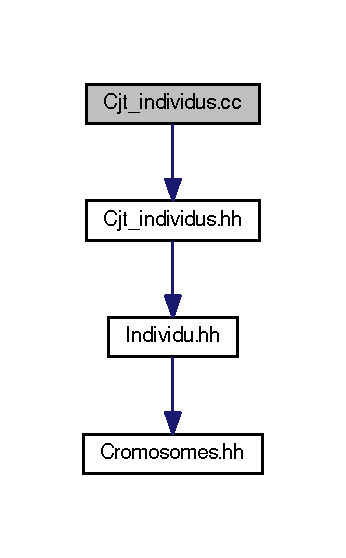
\includegraphics[width=166pt]{_cjt__individus_8cc__incl}
\end{center}
\end{figure}


\subsection{Descripció Detallada}
Codi de la classe \hyperlink{class_cjt__individus}{Cjt\+\_\+individus}. 


\hypertarget{_cjt__individus_8hh}{}\section{Referència del Fitxer Cjt\+\_\+individus.\+hh}
\label{_cjt__individus_8hh}\index{Cjt\+\_\+individus.\+hh@{Cjt\+\_\+individus.\+hh}}


Especificació de la classe \hyperlink{class_cjt__individus}{Cjt\+\_\+individus}.  


Inclou el graf de dependències per a Cjt\+\_\+individus.\+hh\+:
\nopagebreak
\begin{figure}[H]
\begin{center}
\leavevmode
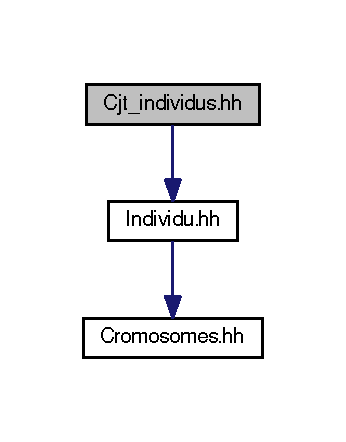
\includegraphics[width=166pt]{_cjt__individus_8hh__incl}
\end{center}
\end{figure}
\subsection*{Classes}
\begin{DoxyCompactItemize}
\item 
class \hyperlink{class_cjt__individus}{Cjt\+\_\+individus}
\begin{DoxyCompactList}\small\item\em Representa el conjunt d\textquotesingle{}individus d\textquotesingle{}un experiment. \end{DoxyCompactList}\end{DoxyCompactItemize}


\subsection{Descripció Detallada}
Especificació de la classe \hyperlink{class_cjt__individus}{Cjt\+\_\+individus}. 


\hypertarget{_cjt__trets_8cc}{}\section{Referència del Fitxer Cjt\+\_\+trets.\+cc}
\label{_cjt__trets_8cc}\index{Cjt\+\_\+trets.\+cc@{Cjt\+\_\+trets.\+cc}}


Codi de la classe \hyperlink{class_cjt__trets}{Cjt\+\_\+trets}.  


Inclou el graf de dependències per a Cjt\+\_\+trets.\+cc\+:
\nopagebreak
\begin{figure}[H]
\begin{center}
\leavevmode
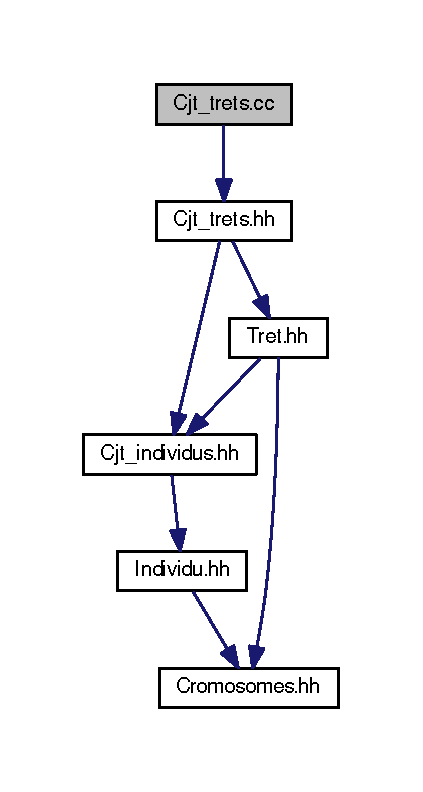
\includegraphics[width=203pt]{_cjt__trets_8cc__incl}
\end{center}
\end{figure}


\subsection{Descripció Detallada}
Codi de la classe \hyperlink{class_cjt__trets}{Cjt\+\_\+trets}. 


\hypertarget{_cjt__trets_8hh}{}\section{Referència del Fitxer Cjt\+\_\+trets.\+hh}
\label{_cjt__trets_8hh}\index{Cjt\+\_\+trets.\+hh@{Cjt\+\_\+trets.\+hh}}


Especificació de la classe \hyperlink{class_cjt__trets}{Cjt\+\_\+trets}.  


Inclou el graf de dependències per a Cjt\+\_\+trets.\+hh\+:
\nopagebreak
\begin{figure}[H]
\begin{center}
\leavevmode
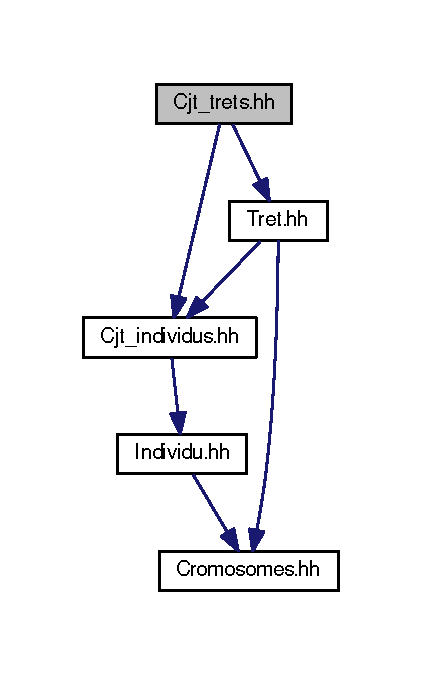
\includegraphics[width=203pt]{_cjt__trets_8hh__incl}
\end{center}
\end{figure}
\subsection*{Classes}
\begin{DoxyCompactItemize}
\item 
class \hyperlink{class_cjt__trets}{Cjt\+\_\+trets}
\begin{DoxyCompactList}\small\item\em Representa el conjunt de trets d\textquotesingle{}un experiment. \end{DoxyCompactList}\end{DoxyCompactItemize}


\subsection{Descripció Detallada}
Especificació de la classe \hyperlink{class_cjt__trets}{Cjt\+\_\+trets}. 


\hypertarget{_cromosomes_8cc}{}\section{Referència del Fitxer Cromosomes.\+cc}
\label{_cromosomes_8cc}\index{Cromosomes.\+cc@{Cromosomes.\+cc}}


Codi de la classe \hyperlink{class_cromosomes}{Cromosomes}.  


Inclou el graf de dependències per a Cromosomes.\+cc\+:
\nopagebreak
\begin{figure}[H]
\begin{center}
\leavevmode
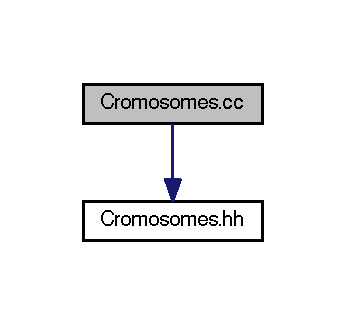
\includegraphics[width=166pt]{_cromosomes_8cc__incl}
\end{center}
\end{figure}


\subsection{Descripció Detallada}
Codi de la classe \hyperlink{class_cromosomes}{Cromosomes}. 


\hypertarget{_cromosomes_8hh}{}\section{Referència del Fitxer Cromosomes.\+hh}
\label{_cromosomes_8hh}\index{Cromosomes.\+hh@{Cromosomes.\+hh}}


Especificació de la classe \hyperlink{class_cromosomes}{Cromosomes}.  


\subsection*{Classes}
\begin{DoxyCompactItemize}
\item 
class \hyperlink{class_cromosomes}{Cromosomes}
\begin{DoxyCompactList}\small\item\em Representa el parell de cromosomes. \end{DoxyCompactList}\end{DoxyCompactItemize}


\subsection{Descripció Detallada}
Especificació de la classe \hyperlink{class_cromosomes}{Cromosomes}. 


\hypertarget{_individu_8cc}{}\section{Referència del Fitxer Individu.\+cc}
\label{_individu_8cc}\index{Individu.\+cc@{Individu.\+cc}}


Codi de la classe \hyperlink{class_individu}{Individu}.  


Inclou el graf de dependències per a Individu.\+cc\+:
\nopagebreak
\begin{figure}[H]
\begin{center}
\leavevmode
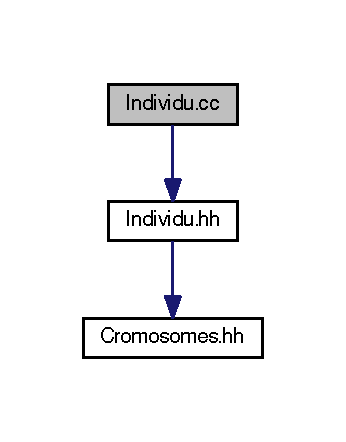
\includegraphics[width=166pt]{_individu_8cc__incl}
\end{center}
\end{figure}


\subsection{Descripció Detallada}
Codi de la classe \hyperlink{class_individu}{Individu}. 


\hypertarget{_individu_8hh}{}\section{Referència del Fitxer Individu.\+hh}
\label{_individu_8hh}\index{Individu.\+hh@{Individu.\+hh}}


Especificació de la classe \hyperlink{class_individu}{Individu}.  


Inclou el graf de dependències per a Individu.\+hh\+:
\nopagebreak
\begin{figure}[H]
\begin{center}
\leavevmode
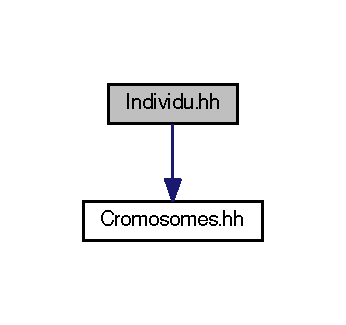
\includegraphics[width=166pt]{_individu_8hh__incl}
\end{center}
\end{figure}
\subsection*{Classes}
\begin{DoxyCompactItemize}
\item 
class \hyperlink{class_individu}{Individu}
\begin{DoxyCompactList}\small\item\em Representa les característiques d\textquotesingle{}un individu. \end{DoxyCompactList}\end{DoxyCompactItemize}


\subsection{Descripció Detallada}
Especificació de la classe \hyperlink{class_individu}{Individu}. 


\hypertarget{program_8cc}{}\section{Referència del Fitxer program.\+cc}
\label{program_8cc}\index{program.\+cc@{program.\+cc}}


Programa principal {\itshape Aplicació per a un laboratori de biologia}.  


Inclou el graf de dependències per a program.\+cc\+:
\nopagebreak
\begin{figure}[H]
\begin{center}
\leavevmode
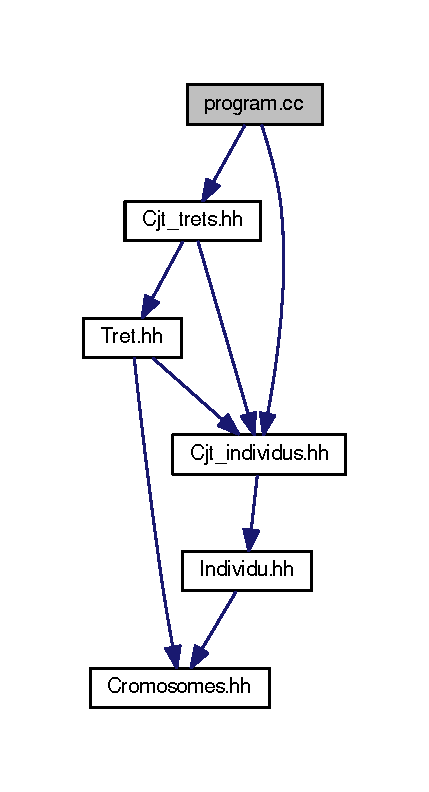
\includegraphics[width=206pt]{program_8cc__incl}
\end{center}
\end{figure}
\subsection*{Funcions}
\begin{DoxyCompactItemize}
\item 
int \hyperlink{program_8cc_ae66f6b31b5ad750f1fe042a706a4e3d4}{main} ()
\end{DoxyCompactItemize}


\subsection{Descripció Detallada}
Programa principal {\itshape Aplicació per a un laboratori de biologia}. 



\subsection{Documentació de les Funcions}
\index{program.\+cc@{program.\+cc}!main@{main}}
\index{main@{main}!program.\+cc@{program.\+cc}}
\subsubsection[{\texorpdfstring{main()}{main()}}]{\setlength{\rightskip}{0pt plus 5cm}int main (
\begin{DoxyParamCaption}
{}
\end{DoxyParamCaption}
)}\hypertarget{program_8cc_ae66f6b31b5ad750f1fe042a706a4e3d4}{}\label{program_8cc_ae66f6b31b5ad750f1fe042a706a4e3d4}


Definició a la línia 20 del fitxer program.\+cc.


\begin{DoxyCode}
20            \{
21   \hyperlink{class_cjt__individus}{Cjt\_individus} i;
22   \hyperlink{class_cjt__trets}{Cjt\_trets} t;
23   \textcolor{keywordtype}{string} op; \textcolor{comment}{// Nom de les operacions}
24   cin >> op;
25   \textcolor{keywordflow}{while}(op!=\textcolor{stringliteral}{"fi"}) \{
26     \textcolor{keywordtype}{string} tret; \textcolor{comment}{// Nom del tret}
27     \textcolor{keywordtype}{int} id, n, m; \textcolor{comment}{// Identificador, nombre d'invidus i nombre de gens}
28     
29     \textcolor{keywordflow}{if}(op==\textcolor{stringliteral}{"experiment"}) \{
30       cin >> n >> m;
31       i.\hyperlink{class_cjt__individus_a478b829d6a11c5259a36a8bd53662e7d}{llegir}(n, m);
32       cout << op << \textcolor{charliteral}{' '} << n << \textcolor{charliteral}{' '} << m << endl;
33     \}
34     \textcolor{keywordflow}{else} \textcolor{keywordflow}{if}(op==\textcolor{stringliteral}{"afegir"}) \{
35       cin >> tret >> id;
36       cout << op << \textcolor{charliteral}{' '} << tret << \textcolor{charliteral}{' '} << \textcolor{keywordtype}{id} << endl;
37       \textcolor{keywordflow}{if}(i.\hyperlink{class_cjt__individus_ab7ef8ea63550958f2025a684dc804308}{individu\_te\_tret}(\textcolor{keywordtype}{id}, tret)) cout << \textcolor{stringliteral}{"  error"} << endl;
38       \textcolor{keywordflow}{else} t.\hyperlink{class_cjt__trets_ad315f780dfe22f6730ee9ce9aa2b25d7}{afegir}(tret, \textcolor{keywordtype}{id}, i);
39     \}
40     \textcolor{keywordflow}{else} \textcolor{keywordflow}{if}(op==\textcolor{stringliteral}{"treure"}) \{
41       cin >> tret >> id;
42       cout << op << \textcolor{charliteral}{' '} << tret << \textcolor{charliteral}{' '} << \textcolor{keywordtype}{id} << endl;
43       \textcolor{keywordflow}{if}(!i.\hyperlink{class_cjt__individus_ab7ef8ea63550958f2025a684dc804308}{individu\_te\_tret}(\textcolor{keywordtype}{id}, tret)) cout << \textcolor{stringliteral}{"  error"} << endl;
44       \textcolor{keywordflow}{else} t.\hyperlink{class_cjt__trets_ae4152db728b8c78d6e56856e0e88de33}{treure}(tret, \textcolor{keywordtype}{id}, i);
45     \}
46     \textcolor{keywordflow}{else} \textcolor{keywordflow}{if}(op==\textcolor{stringliteral}{"consulta\_tret"}) \{
47       cin >> tret;
48       cout << op << \textcolor{charliteral}{' '} << tret << endl;
49       \textcolor{keywordflow}{if}(!t.\hyperlink{class_cjt__trets_a6da10e61a25071a25eca708f61a1e33d}{existeix\_tret}(tret)) cout << \textcolor{stringliteral}{"  error"} << endl;
50       \textcolor{keywordflow}{else} t.\hyperlink{class_cjt__trets_ad53ad0f5574d551fdbc8f665323a1db7}{escriure\_tret}(tret);
51     \}
52     \textcolor{keywordflow}{else} \textcolor{keywordflow}{if}(op==\textcolor{stringliteral}{"consulta\_individu"}) \{
53       cin >> id;
54       cout << op << \textcolor{charliteral}{' '} << \textcolor{keywordtype}{id} << endl;
55       i.\hyperlink{class_cjt__individus_aafb2e0f4456390cbe83009aa542b0991}{escriure}(\textcolor{keywordtype}{id});
56     \}
57     \textcolor{keywordflow}{else} \textcolor{keywordflow}{if}(op==\textcolor{stringliteral}{"distribucio\_tret"}) \{
58       cin >> tret;
59       cout << op << \textcolor{charliteral}{' '} << tret << endl;
60       \textcolor{keywordflow}{if}(!t.\hyperlink{class_cjt__trets_a6da10e61a25071a25eca708f61a1e33d}{existeix\_tret}(tret)) cout << \textcolor{stringliteral}{"  error"} << endl;
61       \textcolor{keywordflow}{else} i.\hyperlink{class_cjt__individus_afbd2a5f911caa9d9ca05470781c395a2}{escriure\_distribucio\_tret}(tret);
62     \}
63     cin >> op;
64   \}
65   cout << \textcolor{stringliteral}{"fi"} << endl;
66 \}
\end{DoxyCode}

\hypertarget{_tret_8cc}{}\section{Referència del Fitxer Tret.\+cc}
\label{_tret_8cc}\index{Tret.\+cc@{Tret.\+cc}}


Codi de la classe \hyperlink{class_tret}{Tret}.  


Inclou el graf de dependències per a Tret.\+cc\+:
\nopagebreak
\begin{figure}[H]
\begin{center}
\leavevmode
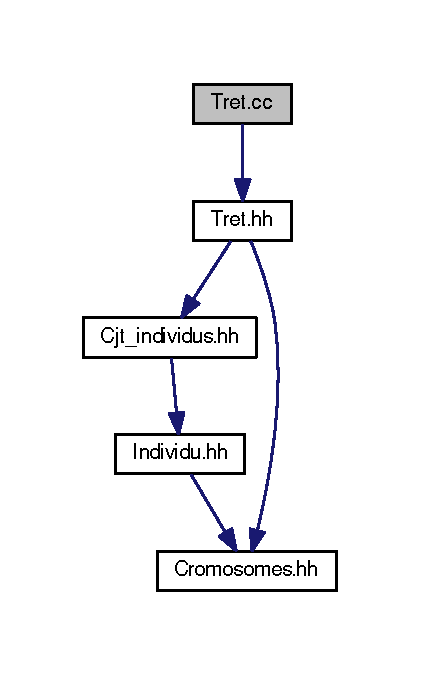
\includegraphics[width=202pt]{_tret_8cc__incl}
\end{center}
\end{figure}


\subsection{Descripció Detallada}
Codi de la classe \hyperlink{class_tret}{Tret}. 


\hypertarget{_tret_8hh}{}\section{Referència del Fitxer Tret.\+hh}
\label{_tret_8hh}\index{Tret.\+hh@{Tret.\+hh}}


Especificació de la classe \hyperlink{class_tret}{Tret}.  


Inclou el graf de dependències per a Tret.\+hh\+:
\nopagebreak
\begin{figure}[H]
\begin{center}
\leavevmode
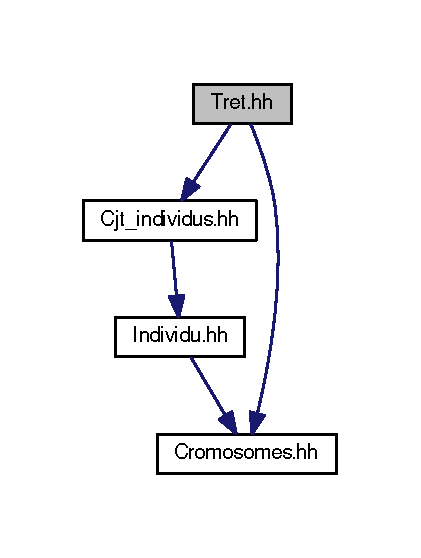
\includegraphics[width=202pt]{_tret_8hh__incl}
\end{center}
\end{figure}
\subsection*{Classes}
\begin{DoxyCompactItemize}
\item 
class \hyperlink{class_tret}{Tret}
\begin{DoxyCompactList}\small\item\em Representa l\textquotesingle{}informació i les operacions associades a un tret. \end{DoxyCompactList}\end{DoxyCompactItemize}


\subsection{Descripció Detallada}
Especificació de la classe \hyperlink{class_tret}{Tret}. 


%--- End generated contents ---

% Index
\backmatter
\newpage
\phantomsection
\clearemptydoublepage
\addcontentsline{toc}{chapter}{Índex}
\printindex

\end{document}
